\documentclass[12pt]{article}
\usepackage[switch, modulo]{lineno}
\usepackage[utf8]{inputenc}
\usepackage[normalem]{ulem} %for strikeout
\usepackage{amsmath}
\usepackage{amsfonts}
\usepackage{amssymb}
\usepackage{bm}
\usepackage{graphicx}
\graphicspath{{Figures/}{figures/}}
\usepackage[superscript,biblabel]{cite}
\usepackage[font={small}]{caption}
\usepackage{tabularx}
\usepackage{subfig}
\usepackage{listings}
\usepackage{courier}
\usepackage{booktabs}
\usepackage{abstract,lipsum}
\usepackage{soul}
\usepackage{multicol}
\usepackage{authblk}
\usepackage{upgreek} %%% This package provides non-italic greek letters: \upalpha, \upbeta or \Upalpha, \Upbeta for uppercase.
\usepackage{algorithm}
\usepackage{algpseudocode}
\newtheorem{theorem}{Theorem}
\newtheorem{proposition}[theorem]{Proposition}
\newtheorem{corollary}[theorem]{Corollary}
\newtheorem{remark}[theorem]{Remark}
\newtheorem{example}[theorem]{Example}
\makeatletter
\def\BState{\State\hskip-\ALG@thistlm}
\makeatother
\newcommand{\tabitem}{~~\llap{\textbullet}~~}
\newcolumntype{L}[1]{>{\raggedright\arraybackslash}X}%
\newcolumntype{R}[1]{>{\raggedleft\arraybackslash}X}%
\newcolumntype{C}[1]{>{\centering\arraybackslash}X}%
%%% Control line spacing
\usepackage{setspace} \doublespacing
\usepackage[font=doublespacing]{caption}
%%% Control text dimensions
\usepackage[margin=1in]{geometry}
\newenvironment{Figure} {\par\medskip\noindent\minipage{0.8\linewidth}} {\endminipage\par\medskip}
%%% Colors
\usepackage{xcolor}
\usepackage{hyperref}
\definecolor{crebuttal}{rgb}{0.33,0.42,0.18} %%% rebuttal color (DarkOlive --> 0.33, 0.42, 0.18).
\definecolor{Kevin}{rgb}{1,0,0}
\DeclareMathOperator\erf{erf}

%%% Draft markup
\newcommand{\note}[1]{{\color{red}\textbf{[NOTE: #1]}}}
\newcommand{\todo}[1]{{\color{blue}\textbf{[TODO: #1]}}}
\newcommand{\prelim}[1]{{\color{orange!80!black}#1}}

% ---------------------------------------------------------------------
% DRAFT NOTES (not printed)
% Orange (\prelim) = preliminary numbers from code/experiments, regenerate before submission.
% Red (\note) = inconsistencies found in the source notes. Blue (\todo) = missing pieces.
% \noindent\fbox{\parbox{0.97\linewidth}{\small
% \textbf{About this draft.} Assembled in October 2026 from the project notes:
% \begin{itemize}\setlength\itemsep{0pt}
% \item \emph{Impact of Phage-Host Morphology on Adsorption Rates} (adsorption survey and encounter-rate models);
% \item \emph{The effect of bacteria motility on the surface attachment of bacteriophage} (rest-frame Brownian dynamics, Stokes flow, event-driven collisions);
% \item \emph{Hydrodynamic Foundations and Validation Framework for Lattice Boltzmann Modeling};
% \item \emph{Phage--Receptor First Passage Times} (supplement);
% \item the Phage-Bacteria ``Junkyard'' notes (CTRW, run-and-tumble, encounter estimators);
% \item the July 2026 update slides (receptor surface model, tail--receptor binding, tethering).
% \end{itemize}
% Numbers in \prelim{orange} come from short preliminary runs of the Python code in \texttt{code/experiments} (Oct 2026) and must be regenerated before submission. \note{} marks inconsistencies found in the source notes, and \todo{} marks missing pieces. Material not used here (multigrid solvers, population-level agent-based model, mucus subdiffusion) is listed in the Supplement, Sec.~S7.}}
% ---------------------------------------------------------------------

\begin{document}

\title{Tail length and the attachment of bacteriophage to a swimming bacterium:\\ a multiscale model from flagellar hydrodynamics to receptor binding}
\date{\today}
\author[1,2,*]{Kevin L. Joiner}
\author[3,4]{Antoni Luque}
\affil[1]{Computational Science Research Center, San Diego State University, San Diego, CA 92182, USA}
\affil[2]{Naval Information Warfare Center, San Diego, CA 92152, USA}
\affil[3]{Department of Mathematics and Statistics, San Diego State University, San Diego, CA 92182, USA}
\affil[4]{Viral Information Institute, San Diego State University, San Diego, CA 92182, USA}
\affil[*]{kevin.l.joiner1@navy.mil}
\setcounter{Maxaffil}{0}
\renewcommand\Affilfont{\itshape\small}

\maketitle
\clearpage

% =====================================================================
\begin{abstract}
Tailed bacteriophages carry tails from about 15\,nm long in podoviruses to more than 150\,nm in sipho- and myoviruses. We do not know whether a longer tail helps a phage adsorb to its host faster. A phage adsorbs in two steps. First it meets the cell, and when the bacterium swims, its swimming sets how often this happens. Then the phage moves over the cell surface until its tail grips a receptor. We model both steps for T4-like phage around a swimming \textit{Escherichia coli}. A lattice Boltzmann model of a rotating body and a helical flagellar bundle (TIGER) gives the flow around the cell. Phages diffuse and drift in this flow, and we track each time one hits the cell. After contact, the phage walks over a capsule-shaped cell that carries a helical band of receptors. When its tail reaches a receptor, the tail binds and tethers the phage to the cell. Single-molecule force measurements set the stiffness of the tether, and a first-passage calculation gives how long the bond lasts. We test the model against 66 adsorption rate constants from 21 studies, which cover 25 phages and 4 host families. \todo{Results summary: how encounter rate, binding probability and time-to-bind scale with tail length, static vs swimming, and how this compares with the survey.}
\end{abstract}

\noindent\textbf{Keywords:} bacteriophage adsorption; tail length; bacterial motility; lattice Boltzmann method; encounter rate; first-passage time.
%

% =====================================================================
\section*{Introduction}
\linenumbers

\paragraph{Adsorption is the gatekeeper of the phage life cycle.} Bacteriophages are the most abundant biological entities on Earth and shape bacterial populations, genomes and biogeochemical cycles. Every lytic cycle has three steps: adsorption to a host, infection, and release of progeny\cite{shao2008bacteriophage,adams1959bacteriophages}. The faster a phage adsorbs, the less time it spends exposed to decay in the environment and the shorter its life cycle\cite{murray1992viral,shao2008bacteriophage}.

About 96\% of phages examined by electron microscopy carry a tail, which recognizes the host and delivers the genome. The tail varies enormously across the three classical morphological families:
\begin{itemize}\setlength\itemsep{0pt}
\item short, non-contractile tails in podoviruses;
\item long, flexible, non-contractile tails in siphoviruses;
\item long, contractile tails in myoviruses.
\end{itemize}

\paragraph{Encounter and attachment are distinct problems.} Adsorption is usually split into two steps. The first is a three-dimensional encounter between virion and cell. The second is a quasi two-dimensional search of the cell surface, ending in reversible and then irreversible binding to a receptor\cite{schwartz1976adsorption,berg1977physics,storms2015modeling}.

\emph{Encounter.} Phages are not motile, but many bacteria are, and swimming dominates the encounter. Our earlier agent-based study showed that for a run-and-tumble \textit{E.~coli} the encounter kernel is set by bacterial motility and is almost independent of phage diffusion, even when the phage subdiffuses in mucus\cite{joiner2019impact}. In the ballistic regime, when the run length is much larger than the contact radius, the kernel is $\beta_{\rm ball}=\pi R_C^2 v_B$\cite{visser2006plankton,kiorboe2008mechanistic}. A longer tail enlarges the contact radius $R_C=R_B+R_P+L_{\rm tail}$, so the encounter kernel should grow with tail length, quadratically when the cell swims.

\emph{Attachment.} After contact, the virion must find a receptor before it diffuses away. Classical treatments model the receptors as absorbing patches on a reflecting sphere\cite{berg1977physics}. They predict a binding probability that saturates with receptor number, and a surface search time that depends on receptor size and density\cite{berg1977physics,schwartz1976adsorption}. Recent structural work shows that the T4 long tail fibres stay folded against the sheath until the virion engages the surface, which is consistent with a virion that walks across the cell surface before committing to infection\cite{hu2015structural}.

\paragraph{Hydrodynamics near a swimming cell is not just Stokes flow past a sphere.} Most encounter models treat the bacterium as a sphere translating through a quiescent fluid. A swimming \textit{E.~coli} is force- and torque-free: the flagellar bundle rotates one way and the body counter-rotates\cite{berg2004coli,lauga2016bacterial}. Time-averaged flow fields around model \textit{E.~coli} show a strong azimuthal (swirling) component around the swimming axis near the body\cite{watari2010hydrodynamics,lauga2016bacterial}. This raises the question of whether the swirl carries phage across the cell surface, and so contributes to the surface search, rather than only bringing them into contact.

\paragraph{The data are ambiguous.} Our survey of literature adsorption rates (Methods) finds a clear difference in tail length between podoviruses and the two long-tailed families. However, the adsorption rates are distributed broadly within every family. The host appears to explain more of the variance than the tail, and for several host groups the measured rate falls well below the ballistic encounter limit. Together these point to attachment efficiency, not encounter, as the step that limits adsorption\cite{edwards2021making}.

\paragraph{This study.} We ask how tail length affects (i) the encounter rate and (ii) the probability and speed of binding, for phage around a swimming bacterium. To do so we combine a resolved model of the flow around the swimmer with a receptor-level model of the surface search and binding. Specifically:
\begin{enumerate}\setlength\itemsep{0pt}
\item We compute the flow around a swimming \textit{E.~coli} with a lattice Boltzmann model (TIGER), validated against canonical Stokes flows.
\item We transport phage in that flow with Brownian dynamics in the cell's rest frame.
\item We resolve the post-contact search on a capsule-shaped cell with explicit receptors.
\item We model tail--receptor binding and tethering using measured gp37--LPS force curves, and derive bond lifetimes from first-passage theory.
\item We compare the resulting tail-length dependence with a curated literature dataset.
\end{enumerate}

% =====================================================================
\section*{Methods}

\subsection*{Overview of the multiscale framework}
The model couples four levels (Fig.~\ref{fig:framework}):
\begin{enumerate}\setlength\itemsep{0pt}
\item \textbf{Fluid.} A steady or time-averaged flow field $\bm u(\bm x)$ around the swimming cell, either analytic (Stokes) or from the TIGER lattice Boltzmann model.
\item \textbf{Transport.} Phage move in $\bm u$ by overdamped Brownian dynamics in the rest frame of the cell, until they contact the cell.
\item \textbf{Surface search.} An attached phage random-walks on a shell around the capsule-shaped cell, which carries $B$ receptors.
\item \textbf{Binding.} A receptor inside the tail cone may bind. A bound phage is tethered by a linear spring that ruptures at a critical force, and the mean bond lifetime follows from a first-passage calculation.
\end{enumerate}
Each simulation step runs these stages in order: compute binding probabilities, compute forces, update positions, apply boundary conditions (Fig.~\ref{fig:framework}B). All code is in the open-source Python package \texttt{tiger} (Software availability).

% ---------------------------------------------------------------------
\subsection*{Fluid flow around the cell}
\paragraph{Low Reynolds number.} For \textit{E.~coli} ($L\sim 1\,\mu$m, $U\sim30\,\mu$m\,s$^{-1}$, $\nu\sim10^{-6}$\,m$^2$\,s$^{-1}$) the Reynolds number is $\mathrm{Re}=UL/\nu\sim3\times10^{-5}$\cite{purcell1977life}. Viscous forces dominate, so the flow follows the swimmer instantly and obeys the Stokes equations\cite{happel1983} (Supplement S1). We compute the flow with the TIGER lattice Boltzmann model (next section), which solves the Navier--Stokes equations and gives Stokes flow at this Reynolds number.

\paragraph{Phages as passive tracers.} Phages are much smaller than the cell and dilute, so they do not change the flow. We treat each phage as a point that the flow carries and that diffuses (one-way coupling). Stokes drag on the capsid, $\gamma=6\pi\eta R_P$, sets the phage diffusion coefficient through the Stokes--Einstein relation (Eq.~\eqref{eq:langevin}) and the relaxation time of the tether.

\paragraph{Analytic baseline.} As a check on the LBM field we also use the Stokes flow past a sphere of radius $R_B$ that translates with velocity $\bm v_B$,
\begin{equation}\label{eq:stokes_sphere}
\bm u_s(\bm r)=\bm v_B\left(\frac{3R_B}{4r}+\frac{R_B^{3}}{4r^{3}}\right)+\bm r\,(\bm v_B\cdot\bm r)\left(\frac{3R_B}{4r^{3}}-\frac{3R_B^{3}}{4r^{5}}\right),
\end{equation}
where $\bm r$ is measured from the sphere centre. In the frame of the cell, phages move with $\bm u_s-\bm v_B$. We use the sphere with the same volume as the capsule, $R_B^{\rm eq}=1.18\,\mu$m. This flow has no rotation of the body or the flagellar bundle. Experiments E2, E3 and E6 use it as the default flow (\texttt{tiger.flow.StokesSwimmerFlow}).

% ---------------------------------------------------------------------
\subsection*{Lattice Boltzmann model of the swimming cell (TIGER)}
\paragraph{Lattice Boltzmann formulation.} The flow around the swimmer is computed with a single-relaxation-time (BGK) lattice Boltzmann method on a D3Q19 lattice\cite{qian1992lattice,kruger2017lbm}. The fluid is represented by populations $f_i(\bm x,t)$ moving with discrete velocities $\bm c_i$ ($i=0,\dots,18$). Density and momentum are the low-order moments
\begin{equation}
\rho=\sum_i f_i,\qquad \rho\bm u=\sum_i f_i\bm c_i+\tfrac{\Delta t}{2}\bm F .
\end{equation}
Each time step is a collision followed by streaming,
\begin{align}
f_i^{\star}(\bm x,t)&=f_i-\frac{1}{\tau}\left[f_i-f_i^{\rm eq}(\rho,\bm u)\right]+\left(1-\frac{1}{2\tau}\right)S_i\,\Delta t,\\
f_i(\bm x+\bm c_i\Delta t,t+\Delta t)&=f_i^{\star}(\bm x,t),
\end{align}
where $f_i^{\rm eq}$ is the second-order Maxwell--Boltzmann equilibrium and $S_i$ is the Guo forcing term, which injects the body force $\bm F(\bm x,t)$ exerted by the swimmer on the fluid\cite{guo2002discrete}.

The relaxation time sets the kinematic viscosity, $\nu=c_s^2(\tau-\tfrac12)\Delta t$ with $c_s^2=1/3$. The low-Reynolds-number regime is reached through parameter choice alone: a large $\tau$, and a Mach number $\mathrm{Ma}=U/c_s\ll1$ to keep the flow nearly incompressible. No-slip walls use bounce-back rules, and moving walls use the velocity-corrected bounce-back.

\paragraph{The TIGER swimmer.} The cell (TIGER: Tail-Integrated Grid-Embedded Rigid body) is a rigid body of radius $R_B$ with a rotating helical flagellar bundle. The model is force- and torque-free and contains two force sources:
\begin{itemize}\setlength\itemsep{0pt}
\item \textbf{Helical bundle.} A thrust/torque source whose geometry follows Watari and Larson\cite{watari2010hydrodynamics}: helix radius $0.85\,R_B$, pitch $0.6\,R_B$ per turn, three turns, axial offset $0.6\,R_B$. It rotates at $\omega_{\rm bundle}$.
\item \textbf{Counter-rotating body.} A ring of point torques at radius $0.55\,R_B$ that balances the bundle torque, $\omega_{\rm body}=-\omega_{\rm bundle}$.
\end{itemize}
Forces are spread onto the lattice with a Gaussian kernel of width $3\,\Delta x$, and the body is advected with the local fluid velocity.

Simulation parameters (\texttt{models/tiger\_lbm}):
\begin{itemize}\setlength\itemsep{0pt}
\item grid $96\times64\times64$, $\tau=0.9$, 2000 steps of $\Delta t=0.02$ lattice time units;
\item $R_B=10\,\Delta x$, with $\Delta x=0.1\,\mu$m so that $R_B=1\,\mu$m;
\item the time unit calibrated by matching the measured bundle frequency to 100\,Hz.
\end{itemize}

\paragraph{Validation.} Before use, the LBM is validated against two canonical flows, each targeting one assumption:
\begin{itemize}\setlength\itemsep{0pt}
\item \textbf{Couette flow} (moving wall): a linear velocity profile tests the moving-wall no-slip condition.
\item \textbf{Poiseuille flow} (uniform body force): a parabolic profile tests linear viscous response and the forcing scheme.
\end{itemize}
We treat both as diagnostics of the hydrodynamic assumptions rather than as qualitative agreement checks. \todo{Insert validation figure (Appendix A1--A2 of the LBM note): simulated vs analytic profiles and $L^2$ error vs resolution. Also add a single translating-sphere test against Eq.~\eqref{eq:stokes_sphere}.}

\paragraph{Coupling to phage transport.} The phage model uses the time-averaged TIGER field. It is interpolated trilinearly onto phage positions and rotated so that the swimming axis coincides with the long axis of the capsule. Outside the LBM grid (about $\pm3\,\mu$m around the cell) the field is set to zero. \note{With the current saved run, the calibrated velocities have a median of $\sim\!470\,\mu$m\,s$^{-1}$ near the cell, about $15\times$ the measured swim speed of \textit{E.~coli} (20--30\,$\mu$m\,s$^{-1}$). Until the calibration is resolved, only the \emph{shape} of the LBM field is used, rescaled so that the median speed $1.5$--$3\,\mu$m from the cell centre equals the swim speed (\texttt{tiger.flow.TigerLBMFlow}, \texttt{target\_speed}). Possible causes to check: $\Delta t$ vs.\ the lattice time unit in the calibration, the strength of the forcing, and the small domain ($\pm3\,R_B$ in $y,z$), whose periodic images confine the flow.}

% ---------------------------------------------------------------------
\subsection*{Bacterial motility and phage transport}
\paragraph{Rest-frame formulation.} Simulations run in the rest frame of the bacterium, which sits at the origin. The swimming velocity enters through the flow (Stokes or LBM). When the cell changes direction, the whole phage cloud is rotated so that the run direction stays along the cell axis (Supplement S5). Time is discretized in units of the phage diffusion time, $\Delta t=0.01$\,s\cite{joiner2019impact}. Phages interact with the bacterium but not with each other.

\paragraph{Run-and-tumble.} The bacterium swims at speed $v_B$ for run times drawn from an exponential distribution, $\Phi(\tau_R)=\omega e^{-\omega\tau_R}$, with mean run time $\langle\tau_R\rangle=1/\omega=1$\,s for \textit{E.~coli}\cite{texbook1,berg2004coli}. At the end of a run, the new direction is offset from the old one by at most an angle $\theta$, using
\begin{equation}
v_x\leftarrow r_1(\cos\theta-1)+1,\quad v_y\leftarrow(2r_2-1)\sqrt{1-v_x^2},\quad v_z\leftarrow\pm\sqrt{1-v_x^2-v_y^2},
\end{equation}
with $r_{1,2}\sim\mathrm{U}(0,1)$. This makes $v_x$ uniform on $[\cos\theta,1]$ and avoids the bias toward $\cos\theta\approx1$ that sampling $\theta$ uniformly would produce.

At long times the cell diffuses with
\begin{equation}\label{eq:DB}
D_B=\frac{v_B^2\tau_R}{3(1-\alpha)},
\end{equation}
where $\alpha=\langle\cos\theta\rangle$\cite{texbook1}.

\paragraph{Phage Brownian dynamics.} The phage relaxation time $m_P/6\pi\eta R_P\sim0.3$\,ns is far shorter than any time step, so the inertial term is dropped. Phage positions follow the overdamped Langevin equation
\begin{equation}\label{eq:langevin}
\dot{\bm x}=\bm u(\bm x)+\sqrt{2D_P}\,\bm\xi(t),\qquad D_P=\frac{k_BT}{6\pi\eta R_P},
\end{equation}
where $\bm\xi$ is unit Gaussian white noise. Following Moldovan \textit{et al.}\cite{moldovan2007kinetics}, the diffusivity is set by the capsid, with no significant contribution from the tail.

Eq.~\eqref{eq:langevin} is integrated as
\begin{equation}
\bm x_{n}=\bm x_{n-1}+\bm u(\bm x_{n-1})\Delta t+\sqrt{24D_P\Delta t}\,\bm w_n,
\end{equation}
with $\bm w_n$ uniform on $[-\tfrac12,\tfrac12]^3$, which has variance $2D_P\Delta t$ per axis\cite{grassia1995computer}. Waiting times between jumps can optionally be drawn from a power law, giving a continuous-time random walk that reproduces subdiffusion in mucus\cite{metzler2000random,joiner2019impact} (Supplement S4). In the present study phages diffuse normally.

\paragraph{Collisions with the cell (event-driven).} A step from $\bm r_{i-1}$ (outside the capture sphere of radius $R$) to $\bm r_i$ (inside) is resolved below the time-step scale. Parameterizing $\bm r(\tau)=\bm r_{i-1}+\tau\bm v$ with $\bm v=\bm r_i-\bm r_{i-1}$ and $\tau\in[0,1]$, the contact time $\tau^*$ is the smallest root of
\begin{equation}
\tau^2+2\frac{\bm r_{i-1}\cdot\bm v}{|\bm v|^2}\tau+\frac{|\bm r_{i-1}|^2-R^2}{|\bm v|^2}=0,
\end{equation}
and the contact point is $\bm r_c=\bm r_{i-1}+\tau^*\bm v$. If the phage does not adsorb, the residual $\bm q=\bm r_i-\bm r_c$ is reflected specularly,
\begin{equation}
\bm r_i^{*}=\bm r_i+2\bm q_\perp+\bm u(\bm r_c)(1-\tau^*)\Delta t ,
\end{equation}
where $\bm q_\perp$ is the inward normal component of $\bm q$.

\paragraph{Boundary conditions.} The domain is a periodic cube. A phage leaving through the upstream face is re-inserted with randomized transverse coordinates, which erases any memory of the wake. The cell surface is either fully absorbing (encounter-rate simulations) or reflecting, followed by the surface-search model (attachment simulations).

\paragraph{Encounter kernel estimator.} The encounter kernel is measured as
\begin{equation}\label{eq:beta_est}
\beta=\frac{V}{N_{\rm act}}\frac{N_{\rm enc}}{\Delta t},
\end{equation}
where $N_{\rm enc}$ is the number of phages entering the capture zone during $\Delta t$, $N_{\rm act}$ the number of active phages and $V$ the domain volume. A phage is deactivated after an encounter and reactivated once it is farther than a cut-off distance. Because phages do not interact, $\beta$ estimated from $M=nN$ phages equals the average of $n$ independent runs with $N$ phages each (Supplement S6). Simulations with large phage numbers are therefore an unbiased, lower-variance substitute for repeated runs at physiological concentration.

% ---------------------------------------------------------------------
\subsection*{Encounter-rate theory}
Phage and bacterium are taken to meet when their centres come within the contact radius
\begin{equation}\label{eq:Rc}
R_C=R_B+R_P+L_{\rm tail},
\end{equation}
where $R_B$ and $R_P$ are equivalent-sphere radii, $R=\tfrac12(lw^2)^{1/3}$.

\emph{Ballistic limit.} If the run length is large compared with the contact radius ($v_B\tau_R\gg R_C$), the cell sweeps a cylinder of radius $R_C$, and
\begin{equation}\label{eq:kball}
\beta_{\rm ball}=\pi R_C^{2}v_B .
\end{equation}

\emph{Diffusive limit.} If $v_B\tau_R<R_C$, the relative motion is diffusive with $\mathfrak D=D_B+D_P$, and the Smoluchowski flux to an absorbing sphere gives
\begin{equation}\label{eq:kdiff}
\beta_{\rm diff}(t)=4\pi R_C\mathfrak D\left(1+\frac{R_C}{\sqrt{\pi\mathfrak D t}}\right)\;\xrightarrow{t\to\infty}\;4\pi R_C\mathfrak D .
\end{equation}

Because $\beta_{\rm diff}\le\beta_{\rm ball}$ whenever $v_B\tau_R>R_C$, the ballistic kernel is the maximum achievable encounter rate for a swimming host\cite{visser2006plankton,joiner2019impact}. A tail of length $L$ therefore increases the encounter rate by a factor $(1+L/(R_B+R_P))^2$ in the ballistic regime, and $(1+L/(R_B+R_P))$ in the diffusive regime.

\note{The adsorption-survey draft wrote $\beta_{\rm diff}=\tfrac43\pi R_C\mathfrak D$; the Smoluchowski prefactor is $4\pi$. The \texttt{plot\_fun.m} theory curve in the MATLAB code used $R_C^2/\sqrt{\pi\mathfrak D t}$ for the transient term; the classical term is $R_C/\sqrt{\pi\mathfrak D t}$ as above. Both are corrected here.}

% ---------------------------------------------------------------------
\subsection*{Cell surface and receptor model}
\paragraph{Capsule geometry.} The cell is a capsule (spherocylinder) aligned with the $y$ axis: a cylinder of radius $R_B$ for $|y|\le L_B$, capped by hemispheres centred at $y=\pm L_B$ (Fig.~\ref{fig:receptors}A). The surface is the zero set of the level-set function
\begin{equation}
\phi(\bm x)=|\bm x-\bm c(\bm x)|^2-R_B^2,\qquad \bm c(\bm x)=\big(0,\ \mathrm{clip}(y,-L_B,L_B),\ 0\big),
\end{equation}
with outward normal $\nabla\phi/|\nabla\phi|$.

On the cylinder this reduces to $x^2+z^2=R_B^2$, and on the caps to $x^2+(y\mp L_B)^2+z^2=R_B^2$. We use $R_B=0.8\,\mu$m and $L_B=1.9\,\mu$m, giving a 5.4\,$\mu$m long cell. \note{This is longer than the $\approx2$--$3\,\mu$m \textit{E.~coli} in \texttt{bacteria\_characteristics.xlsx}; reconcile.}

\paragraph{Receptor placement.} $B=1000$ receptors of capture radius $R_r$ are distributed within a helical band of half-thickness $\delta=0.05\,\mu$m and pitch angle $m$. A receptor with helical angle $\theta\sim\mathrm U(0,\theta_{\max})$ and offset $a\sim\mathrm U(-\delta,\delta)$ sits at height
\begin{equation}
y=m\theta+\frac{a+\delta}{\cos m}-(L_B+R_B),\qquad \theta_{\max}=\frac{2(L_B+R_B-\delta/\cos m)}{m}.
\end{equation}
It is mapped to $(R_B\cos\theta,\,y,\,R_B\sin\theta)$ on the cylinder, or to the corresponding latitude on a cap. Receptors closer than $2R_r$ to an existing one are redrawn.

Small $m$ spreads the receptors uniformly over the cell. Increasing $m$ concentrates them in a helical band (Fig.~\ref{fig:receptors}B), mimicking the helical organization of outer-membrane proteins. \todo{Cite the helical receptor organization and justify $B$, $R_r$ for T4 (OmpC/LPS) and lambda (LamB).}

% ---------------------------------------------------------------------
\subsection*{Surface search after contact}
A phage whose bulk step would penetrate the cell becomes \emph{attached}. Its capsid centre is then confined to a shell at distance
\begin{equation}
R_{\rm shell}=R_B+\tfrac12(L_{\rm tail}+R_P)
\end{equation}
from the cell axis, so that the tail tip, inclined against the surface, reaches the outer membrane (Fig.~\ref{fig:tailgeom}A).

Each surface step has two parts.
\begin{enumerate}\setlength\itemsep{0pt}
\item \emph{Tangential kick.} A random tangent vector is built as $\bm v=\hat{\bm n}\times\bm w$ with $\bm w\sim\mathrm U(0,1)^3$. It is scaled to length $\sqrt{24D_P\Delta t}\,(U-\tfrac12)$ and rotated about $\hat{\bm n}$ by a uniform angle (Rodrigues formula).
\item \emph{Projection.} The kicked point $\bm r_1$ is projected back onto the shell along the level-set gradient,
\begin{equation}
\bm r_2=\bm r_1-\phi(\bm r_1)\frac{\nabla\phi(\bm r_1)}{|\nabla\phi(\bm r_1)|^2},
\end{equation}
which follows from a first-order Taylor expansion of $\phi$ about $\bm r_1$. It converges to the exact closest-point projection used in the code.
\end{enumerate}

Over the simulated times, attached phage cover distances of several micrometres on the surface (Fig.~\ref{fig:receptors}C). \todo{Report the surface MSD and compare the effective 2D diffusion coefficient with the bulk $D_P$. Geodesic distances on the capsule (slides 16--17) can be used to measure surface displacement.}

% ---------------------------------------------------------------------
\subsection*{Tail--receptor interaction}
\paragraph{Binding probability.} A receptor can be engaged when it lies within the tail cone. For a tail tilted at $60^\circ$, the base of the cone has radius (Fig.~\ref{fig:tailgeom}B)
\begin{equation}
R_{\rm tail}=\sqrt{(L_{\rm tail}+R_P)^2-\left(\tfrac{L_{\rm tail}+R_P}{2}\right)^2}=\frac{\sqrt3}{2}(L_{\rm tail}+R_P).
\end{equation}
With $n$ receptors of radius $R_r$ inside the cone, the receptor-free fraction of the cone base is
\begin{equation}\label{eq:pnot}
P_{\rm not}=1-n\left(\frac{R_r}{R_{\rm tail}}\right)^2 .
\end{equation}
At each step a uniform number $U$ is drawn. If $U>P_{\rm not}$, one of the $n$ receptors, chosen at random, binds. The per-step binding probability is therefore the covered fraction $n(R_r/R_{\rm tail})^2$. This is the analogue, at the scale of the tail, of the Berg--Purcell capture probability $P=Ns/(Ns+\pi a)$ for $N$ absorbing patches of radius $s$ on a sphere of radius $a$\cite{berg1977physics}.

\note{The MATLAB/Python implementation (\texttt{binding\_fun.m}) differs from the slides in two ways. (i) It binds when $U>n(R_r/R_{\rm cone})^2$, i.e.\ with probability $1-$covered fraction, which is almost certain whenever any receptor is in the cone. (ii) It uses $R_{\rm cone}=L_{\rm tail}+R_P$ without the $\sqrt3/2$ factor. With $R_r=0.1$\,nm and $R_{\rm tail}\sim0.1\,\mu$m, the rule in Eq.~\eqref{eq:pnot} gives per-step probabilities of $\sim\!10^{-6}$ and essentially no binding. Choosing the rule, a physical $R_r$, and possibly a per-encounter rather than per-step probability, is the first open decision (experiment E5).}

\paragraph{Tethering.} Once a receptor binds, the phage head is tethered to it (Fig.~\ref{fig:force}). AFM force spectroscopy of T4 gp37 adhesin on \textit{E.~coli}~B lipopolysaccharide\cite{brzozowska2019} shows a force that is linear in extension up to a first rupture,
\begin{equation}
\bm F=-k_{\rm bind}\,(|\bm p|-R)\,\hat{\bm p}\quad (|\bm p|>R),\qquad \bm F=\bm 0\quad(|\bm p|\le R),
\end{equation}
where $\bm p$ is the receptor-to-phage vector and $R=L_{\rm tail}+R_P$ is the rest length. A linear fit gives $k_{\rm bind}\approx65$\,pN\,nm$^{-1}$, with first rupture at $F_{\rm rup}\approx70\pm29$\,pN about 12.5\,nm from contact\cite{brzozowska2019}, similar to antibody--antigen unbinding curves\cite{hinterdorfer1996detection}.

In the overdamped limit the extension obeys $\gamma\dot{\bm x}=-k_{\rm bind}\bm x+\gamma\bm a$, where $\bm a$ is the imposed drift and $\gamma=6\pi\eta R_P$. The solution
\begin{equation}
\bm x(t)=\frac{\gamma}{k_{\rm bind}}\left(1-e^{-k_{\rm bind}t/\gamma}\right)\bm a
\end{equation}
relaxes on the time scale $t_r=\gamma/k_{\rm bind}\approx3\times10^{-8}$\,s. This is six orders of magnitude below $\Delta t$, so explicit integration is unstable. We therefore either use the exact exponential update above, or enforce the tether and the surface as holonomic constraints with the RATTLE integrator\cite{andersen1983rattle}, with Lennard-Jones repulsion between capsid and receptors (Supplement S3). \note{The tether force is computed but multiplied by zero in the original MATLAB surface walk (\texttt{0*F\_proj}). It is a switch (\texttt{tether\_force\_scale}) in the Python port and is off by default until calibrated.}

% ---------------------------------------------------------------------
\subsection*{Bond lifetime from first-passage times}
A bound phage escapes when thermal fluctuations carry the tether past the rupture point. We treat the tether coordinate $x$ as an overdamped particle in the potential obtained by integrating the measured force curve, $U(x)=-\int F\,dx$. For the linear model, $U=\tfrac12k_{\rm bind}x^2$ for $|x|<x_A$ and flat beyond, where $F(x_A)=F_{\rm rup}$ (Fig.~\ref{fig:force}B).

The probability density $P(x,t)$ obeys the Fokker--Planck equation
\begin{equation}
\frac{\partial P}{\partial t}=\frac{\partial}{\partial x}\left[D\,e^{-\tilde U}\frac{\partial}{\partial x}\left(e^{\tilde U}P\right)\right],\qquad \tilde U=U/k_BT,
\end{equation}
with absorbing boundaries at $\pm x_A$. Laplace-transforming and integrating twice (Supplement S2) shows that the first-passage time is exponentially distributed, $f(t)=\lambda e^{-\lambda t}$, with mean
\begin{equation}\label{eq:mfpt}
\langle t\rangle=\frac{1}{\lambda}=\frac1D\int_{-x_A}^{x_A}e^{-\tilde U(x)}\left(\int_{x}^{x_A}e^{\tilde U(y)}\,dy\right)dx ,
\end{equation}
the Kramers escape time\cite{kramers1940brownian,zwanzig2001nonequilibrium}. Here $D=k_BT/6\pi\eta R_P$ is the diffusivity of the phage head.

Fitting $U/k_BT=a\,[1-\mathrm{sech}(bx)]$ to the integrated force curve gives a well depth of $a\approx2.7\times10^{3}\,k_BT$ and $b\approx0.12$\,nm$^{-1}$. Eq.~\eqref{eq:mfpt} is evaluated numerically for rupture forces of 50--120\,pN.

% ---------------------------------------------------------------------
\subsection*{Literature survey of adsorption rates}
\paragraph{Data compilation.} Adsorption rate constants $k$ (mL\,h$^{-1}$) were compiled from 21 studies, giving 66 measurements for 25 phages: 16 Siphoviridae, 36 Myoviridae, 14 Podoviridae. They cover four host families: Enterobacteriaceae ($n=30$), Synechococcaceae (18), Pseudomonadaceae (12) and Vibrionaceae (6). The dataset (\texttt{data/adsorption\_data.xlsx}) records reference, host, tail family, phage, temperature, and two group codes: \emph{Study} (family $\times$ host) and \emph{Bac type} (host). Sources and URLs are in \texttt{data/adsorption\_references.xlsx}.

Where a study reported the percentage of phage adsorbed, $\Delta\hat P=(P_0-P_{\rm final})/P_0$, after incubation time $t$ with host concentration $B$, it was converted with
\begin{equation}
k=-\frac{1}{tB}\ln\left(1-\Delta\hat P\right),
\end{equation}
taking $B=P_0/\mathrm{MOI}$ when only the multiplicity of infection was given\cite{abedon2023adsorption}.

\paragraph{Phage and host characteristics.} Capsid diameters and tail lengths for Lambda and T1--T7 are taken from published measurements. T6 and the T2 tail are assigned T4 values. For the remaining phages, family-typical medians are drawn from per-family pools, $n=8$--10 values per family: tail length 165.5\,nm (Sipho), 142.5\,nm (Myo), 16.0\,nm (Podo). These are listed in \texttt{data/phage\_characteristics.xlsx}. Host length, width, swim speed and run time are listed in \texttt{data/bacteria\_characteristics.xlsx}; E.~coli swim speed and tumble rate vs temperature are from Maeda \textit{et al.}\cite{maeda1976effect}.

\note{The survey draft's Table~1 reports \emph{means} (Sipho 281\,nm, which includes a 980\,nm outlier; Myo 134; Podo 18.9) labelled as medians, and duplicates the $R_P$ column header. The draft also lists \textit{P.~aeruginosa} at 51.3\,$\mu$m\,s$^{-1}$ while the data sheet uses 7.5\,$\mu$m\,s$^{-1}$, and \textit{E.~coli} at 21 vs 30\,$\mu$m\,s$^{-1}$. Reconcile before regenerating the tables.}

\paragraph{Statistics.} Group differences were tested with two-sided Wilcoxon rank-sum (Mann--Whitney U) tests\cite{mann1947test}. Distributions were reconstructed by non-parametric bootstrap\cite{efron1993bootstrap}: tail and capsid sizes were resampled from each phage's reported values, or from its family pool when no phage-specific value existed. The bootstrapped regression was the z-scored ordinary least squares fit
\begin{equation}
\tilde k=\beta_B\tilde R_B+\beta_T\tilde L_{\rm tail}+\beta_H\tilde R_P+\varepsilon
\end{equation}
on Study-group means, refit on 2000 bootstrap replicates.

\paragraph{Violin plots.} Distributions are displayed as violin plots: a kernel density estimate mirrored about the group axis, overlaid with the individual measurements, the median (white circle) and the interquartile range (bar)\cite{hintze1998violin}. They are drawn on log axes because the rates are strongly right-skewed and span two decades. In the host panel, the ballistic predictions $\beta_{\rm ball}=\pi R_C^2v_B$ are overlaid as open circles with bootstrap intervals.

% ---------------------------------------------------------------------
\subsection*{Simulation experiments}
The experiments in \texttt{code/experiments} are designed around the tail-length question.
\begin{description}\setlength\itemsep{0pt}
\item[E1] Binding vs tail length, static cell. $L_{\rm tail}\in\{10,50,100,200,300\}$\,nm, 100 phages, 2400 steps of 0.01\,s, $\ge5$ replicates. Outputs: fraction attached and bound, first-binding-time survival curves, binding rate.
\item[E2] As E1, with free phage advected by the flow of a cell swimming at 30\,$\mu$m\,s$^{-1}$: Stokes flow past the equal-volume sphere, or the rescaled TIGER LBM field.
\item[E3] Encounter kernel vs tail length and swim speed. Eqs.~\eqref{eq:kball}--\eqref{eq:kdiff} compared with simulations in Stokes flow, with capture at $R_C$ from Eq.~\eqref{eq:Rc}.
\item[E4] Literature comparison: statistics and violin plots of the survey, and kinetic predictors per Study group.
\item[E5] Sensitivity to the binding rule, the tether force, and bond lifetime vs rupture force.
\item[E6] Visualization of phage searching and binding on the rotating TIGER cell.
\end{description}

\subsection*{Software availability}
All models are implemented in the Python package \texttt{tiger}, ported from the original MATLAB code with documented corrections (\texttt{code/archive/PORT\_NOTES.md}). It is accompanied by unit tests of the analytic limits: ballistic kernel, Smoluchowski capture time, run-and-tumble diffusivity, CTRW exponent, Stokes no-slip, and RATTLE constraint conservation. \todo{Repository URL / Zenodo DOI.}

% =====================================================================
\section*{Results}

\subsection*{Adsorption rates in the literature are host-structured, not tail-structured}
\textbf{Tail length.} Tail length differs sharply between families. Podovirus tails (median 16\,nm) are shorter than both siphovirus (165.5\,nm) and myovirus (142.5\,nm) tails (rank-sum $p=7.8\times10^{-4}$ for both comparisons). Sipho and Myo tails are not significantly different ($p=0.16$). Capsid sizes overlap across families (Fig.~\ref{fig:adsorption}A).

\textbf{Adsorption rate.} Adsorption rates span $10^{-8}$--$10^{-6}$\,mL\,h$^{-1}$ within every family (Fig.~\ref{fig:adsorption}B). In the curated 66-measurement dataset, family medians are $2.4\times10^{-7}$ (Sipho), $5.8\times10^{-8}$ (Myo) and $3.6\times10^{-7}$\,mL\,h$^{-1}$ (Podo). The low myovirus median is driven by 16 cyanophage measurements on \textit{Synechococcus}. The rate ranking therefore does not follow tail length: the shortest-tailed family has the highest median.

\textbf{Family tests.} Myo differs from Sipho ($p=0.017$) and from Podo ($p=0.011$; $p=0.052$ without the two Niu 2022 values flagged in the data). Sipho vs Podo is not significant ($p=0.43$).

\textbf{Host.} Broken out by host (Fig.~\ref{fig:adsorption}C,D), Enterobacteriaceae rates (median $1.9\times10^{-7}$) exceed those of Synechococcaceae ($3.9\times10^{-8}$; $p=5.4\times10^{-5}$) and Vibrionaceae ($5.3\times10^{-8}$; $p=3.6\times10^{-3}$). However, they fall below Pseudomonadaceae ($6.0\times10^{-7}$; $p=0.013$).

\textbf{Bootstrap regression.} The bootstrapped regression on Study-group means explains little variance (median $R^2=0.21$). Neither tail length (median $\beta_T=-0.36$, $p=0.39$) nor capsid or host size is a significant predictor.

\note{These numbers come from the cleaned 2026 dataset and \emph{change two conclusions of the earlier survey draft} (57 measurements). That draft found no family differences and \textit{E.~coli} as the top host. In the current data, \textit{Pseudomonas} has higher rates than \textit{E.~coli} (new Namonyo 2023 and Niu 2022 entries), and Myo differs from both other families. The violin figures (Fig.~\ref{fig:adsorption}) are from the earlier dataset and must be regenerated with E4. The data issues listed in \texttt{adsorption\_data.xlsx} should be resolved first, since several of them move rows between families: Koonjan 2021 phage identity, Mann 2003 S-PM vs S-BBS1, Xu/Sillankorva ``T7'', and the Niu 2022 units.}

\subsection*{Measured rates sit below the ballistic encounter limit except for enteric hosts}
\textbf{Regime.} For each host, the contact radius was bootstrapped from Eq.~\eqref{eq:Rc}. The run length $v_B\tau_R$ exceeds $R_C$ by one to two orders of magnitude. The ballistic kernel is therefore the appropriate upper bound, and the run-and-tumble diffusive kernel overestimates it (Table~\ref{tbl:predictors}).

\textbf{Comparison with data.} Measured rates for \textit{Synechococcus} and \textit{Vibrio} fall well below $\beta_{\rm ball}$, which exceeds the 75th percentile of the data. Enteric hosts reach their ballistic limit. \todo{Recompute with reconciled host speeds; the earlier draft's values were $\tilde\beta_{\rm ball}=0.9$--$3.3\times10^{-7}$\,mL\,h$^{-1}$.} This gap between encounter and adsorption is the attachment efficiency the receptor-level model is designed to explain.

\subsection*{Tail length raises the encounter kernel}
In Stokes-flow simulations (E3; \prelim{20{,}000 phages, 600 steps}), the encounter kernel at $v_B=30\,\mu$m\,s$^{-1}$ rises with tail length:
\begin{itemize}\setlength\itemsep{0pt}
\item \prelim{$33\,\mu$m$^3$\,s$^{-1}$ at $L=50$\,nm;}
\item \prelim{$86\,\mu$m$^3$\,s$^{-1}$ at $L=300$\,nm;}
\item \prelim{$137\,\mu$m$^3$\,s$^{-1}$ at $L=500$\,nm.}
\end{itemize}
These values lie below $\beta_{\rm ball}$ and track its quadratic dependence on $R_C$ (Fig.~\ref{fig:prelim}C). For a static cell the dependence is weaker and approaches the Smoluchowski limit $4\pi R_C D_P$.

\note{The kernel for $L\to0$ is underestimated because the capture shell (thickness $R_P=50$\,nm) is thinner than a diffusive step ($\sqrt{24D_P\Delta t}\approx0.6\,\mu$m). Production runs need $\Delta t$ reduced near the cell, or an analytic hitting-probability correction per step.}

\subsection*{Binding vs tail length on a static and a swimming cell}
\prelim{Preliminary (E1/E2, 100 phages, 12\,s, 3 replicates, MATLAB binding rule):}
\begin{itemize}\setlength\itemsep{0pt}
\item \prelim{On a static cell, the bound fraction after 12\,s changes little with tail length (0.48--0.53). The median time to first binding falls from 0.31\,s ($L=10$\,nm) to 0.06\,s ($L=300$\,nm).}
\item \prelim{When the cell swims at 30\,$\mu$m\,s$^{-1}$ (Stokes flow), the bound fraction rises from 0.64 to 0.74 and the binding rate from 0.13 to 0.20\,s$^{-1}$ per phage over the same range (Fig.~\ref{fig:prelim}A,B).}
\end{itemize}
\todo{Full E1/E2 with the resolved binding rule, the TIGER LBM field, $\ge5$ replicates and survival-curve fits. Decompose the tail effect into (i) a larger capture radius, (ii) a larger tail cone with more receptors per search step, and (iii) a different shell radius.}

\subsection*{Tether lifetimes are extremely sensitive to rupture force}
With $k_{\rm bind}=65$\,pN\,nm$^{-1}$, Eq.~\eqref{eq:mfpt} gives mean bond lifetimes rising by about nine orders of magnitude as the rupture force increases from 50 to 120\,pN (Fig.~\ref{fig:force}C). They range from microseconds at $F_{\rm rup}=50$\,pN, to $\sim\!2$\,ms at 79\,pN, to over an hour at 120\,pN. Within the measured range ($70\pm29$\,pN) a single gp37--LPS bond is therefore either transient or effectively permanent on the time scale of the surface search. This argues that multivalent binding by several long tail fibres, not a single bond, sets the transition from reversible to irreversible attachment. \todo{Couple bond lifetime to the surface walk: allow unbinding and rebinding, and count bound fibres.}

% =====================================================================
\section*{Discussion}
\todo{Draft once E1--E3 are final. Points carried over from the notes:}
\begin{itemize}
\item \textbf{Encounter vs attachment.} Encounter models alone predict the upper bound of adsorption. The shortfall in non-enteric hosts points to attachment efficiency as the limiting step. Adsorption should be written as contact rate $\times$ attachment efficiency, where the efficiency depends on receptor availability and affinity and on reversible binding that keeps the virion near the cell\cite{edwards2021making,schwartz1976adsorption}.
\item \textbf{Tail length.} A longer tail enlarges the capture radius and the tail cone. The family data nonetheless show no monotone dependence of adsorption on tail length. This is consistent with the observation that irreversible binding, not tail-fibre identity, correlates with infection success.
\item \textbf{Hydrodynamics of the swimmer.} Earlier Stokes-flow simulations in mucus showed phage accumulating at the front of a swimming cell only when the phage also interacted with mucus. The torque-free swirl resolved by TIGER is a candidate for transporting attached phage across the surface, and for re-delivering detached phage. Whether it shortens the search is the central hydrodynamic question here.
\item \textbf{T4 polar preference.} T4 preferentially infects at the cell poles, which suggests that virions move over the surface before committing. Strain on the baseplate from relative motion between phage and cell (convection, Brownian motion, swimming) could promote the transition to irreversible binding.
\item \textbf{Model organisms.} Coliphages may be atypical, fast adsorbers relative to environmental phages (a ``streetlight effect''). The 2026 data, where \textit{Pseudomonas} phages are fastest, complicate that claim, and it should be revisited.
\item \textbf{Limitations.} The analysis assumes a rigid tail, a single receptor type and a single bond, and a time-averaged flow. The binding rule and receptor size are not yet calibrated, and the LBM velocity magnitude is not yet calibrated.
\end{itemize}

% =====================================================================
\clearpage
\begin{spacing}{1.0}
\begin{spacing}{1.0}
\bibliography{references}
\bibliographystyle{unsrt}
\end{spacing}
\newpage
\end{spacing}

% =====================================================================
\clearpage
\section*{Figures and Tables}
\addcontentsline{toc}{section}{Figures and Tables}

\begin{figure}[!ht]
\centering
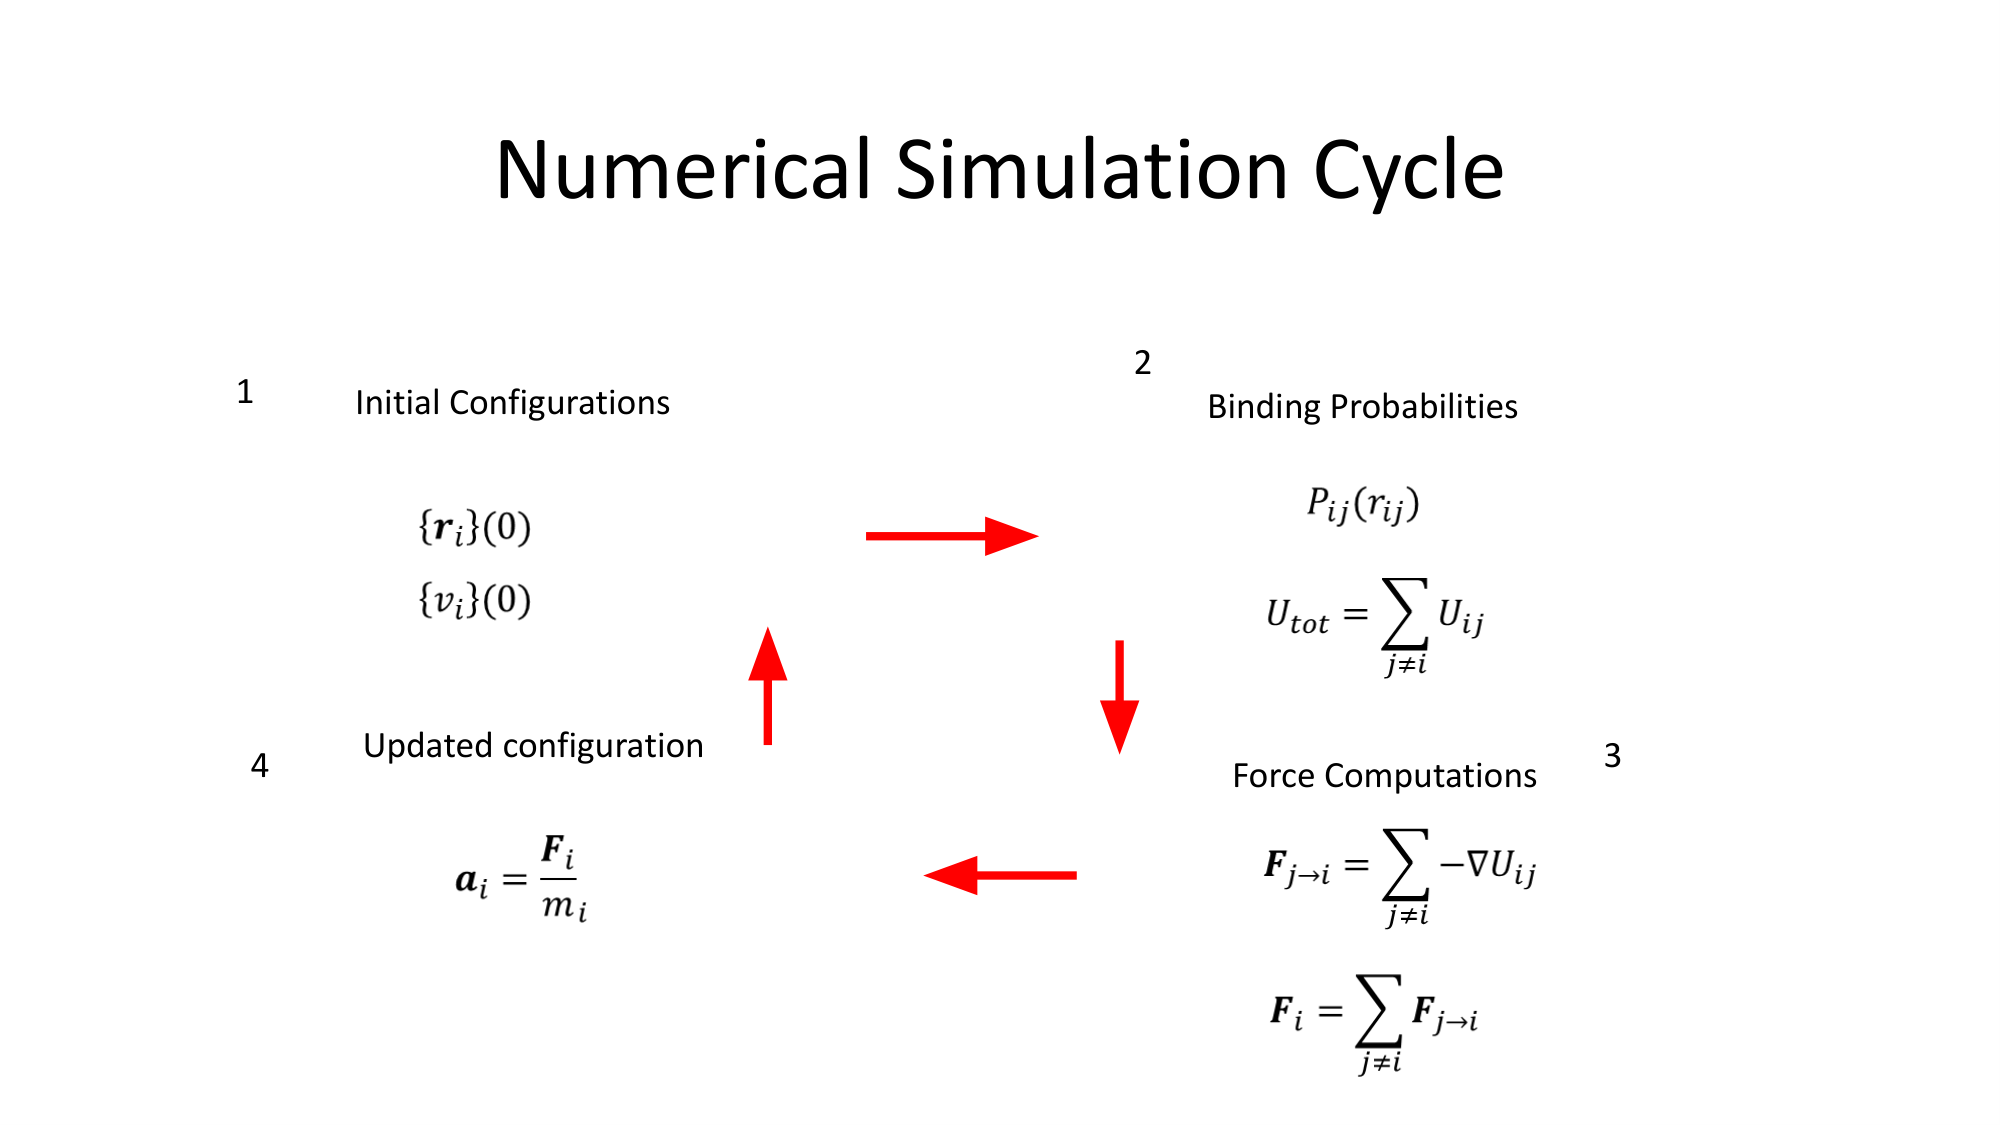
\includegraphics[width=0.48\linewidth]{slide_simulation_cycle.png}\hfill
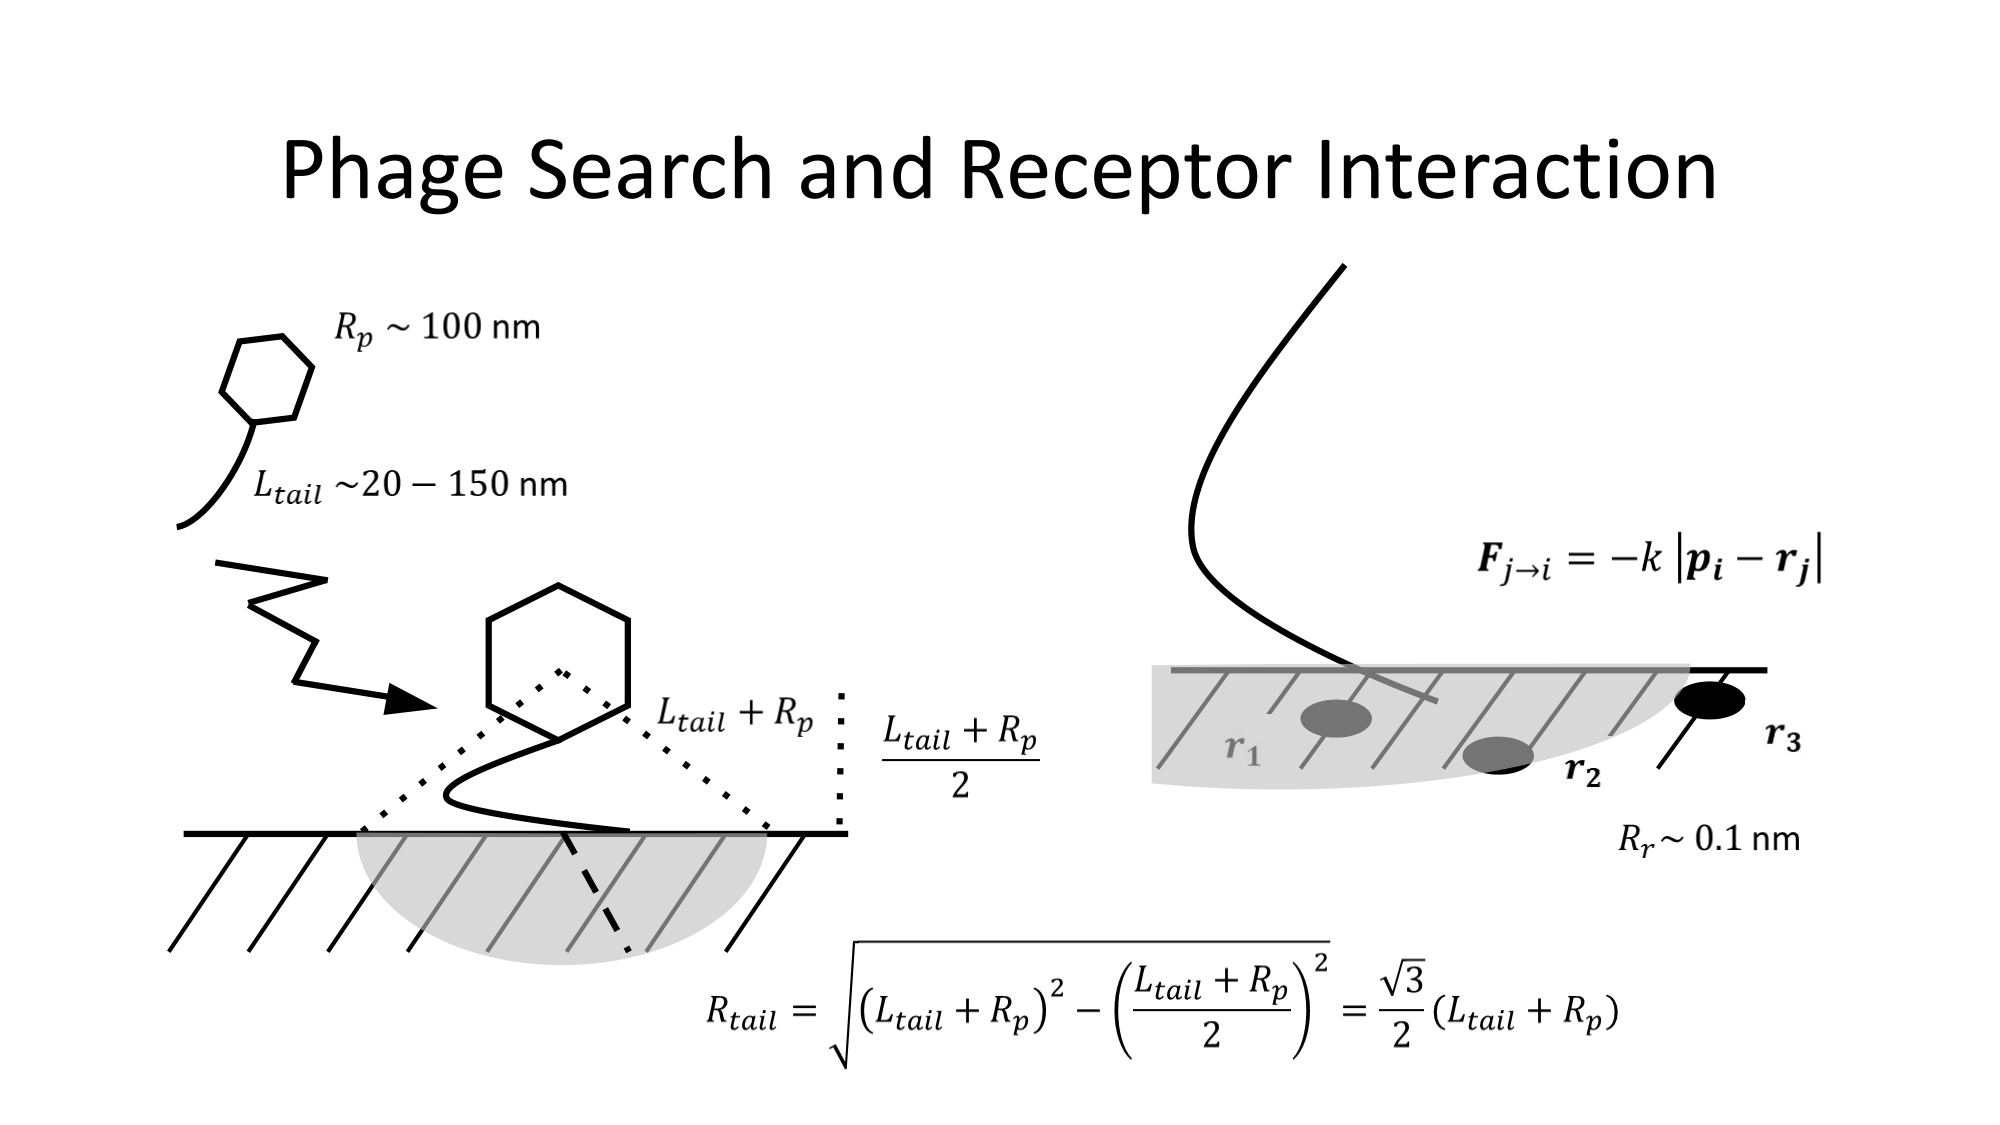
\includegraphics[width=0.48\linewidth]{slide_tail_geometry.png}
\caption{Model framework. (A) Numerical simulation cycle: initial configuration $\to$ binding probabilities $\to$ force computations $\to$ updated configuration. (B) Phage on the cell surface: capsid of radius $R_P\sim100$\,nm and tail of length $L_{\rm tail}\sim20$--150\,nm, centre at $R_B+(L_{\rm tail}+R_P)/2$, tail cone of radius $\tfrac{\sqrt3}{2}(L_{\rm tail}+R_P)$. \todo{Redraw as a single schematic with the TIGER flow field, the surface shell and the tail cone; slides are placeholders.}}
\label{fig:framework}\label{fig:tailgeom}
\end{figure}

\begin{figure}[!ht]
\centering
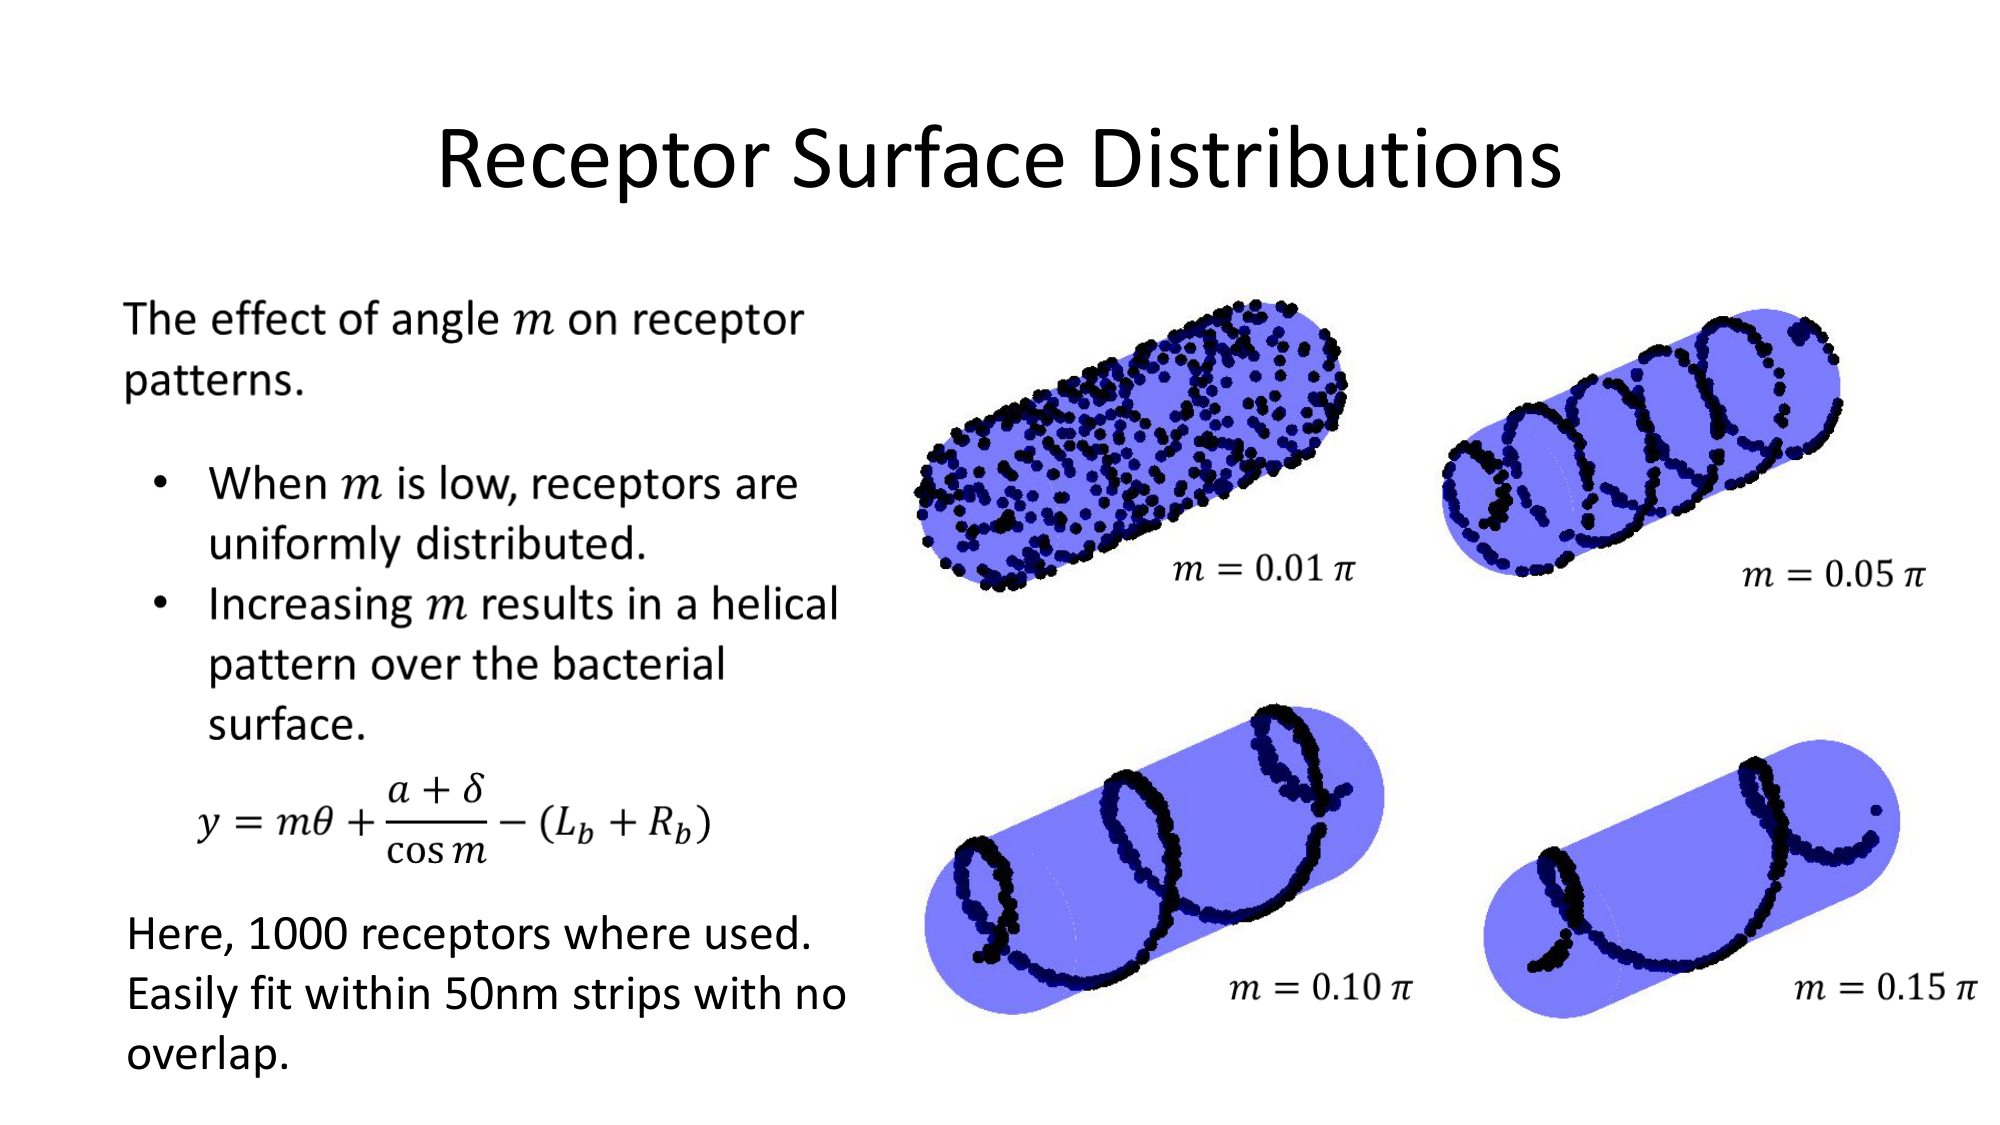
\includegraphics[width=0.48\linewidth]{slide_receptor_distributions.png}\hfill
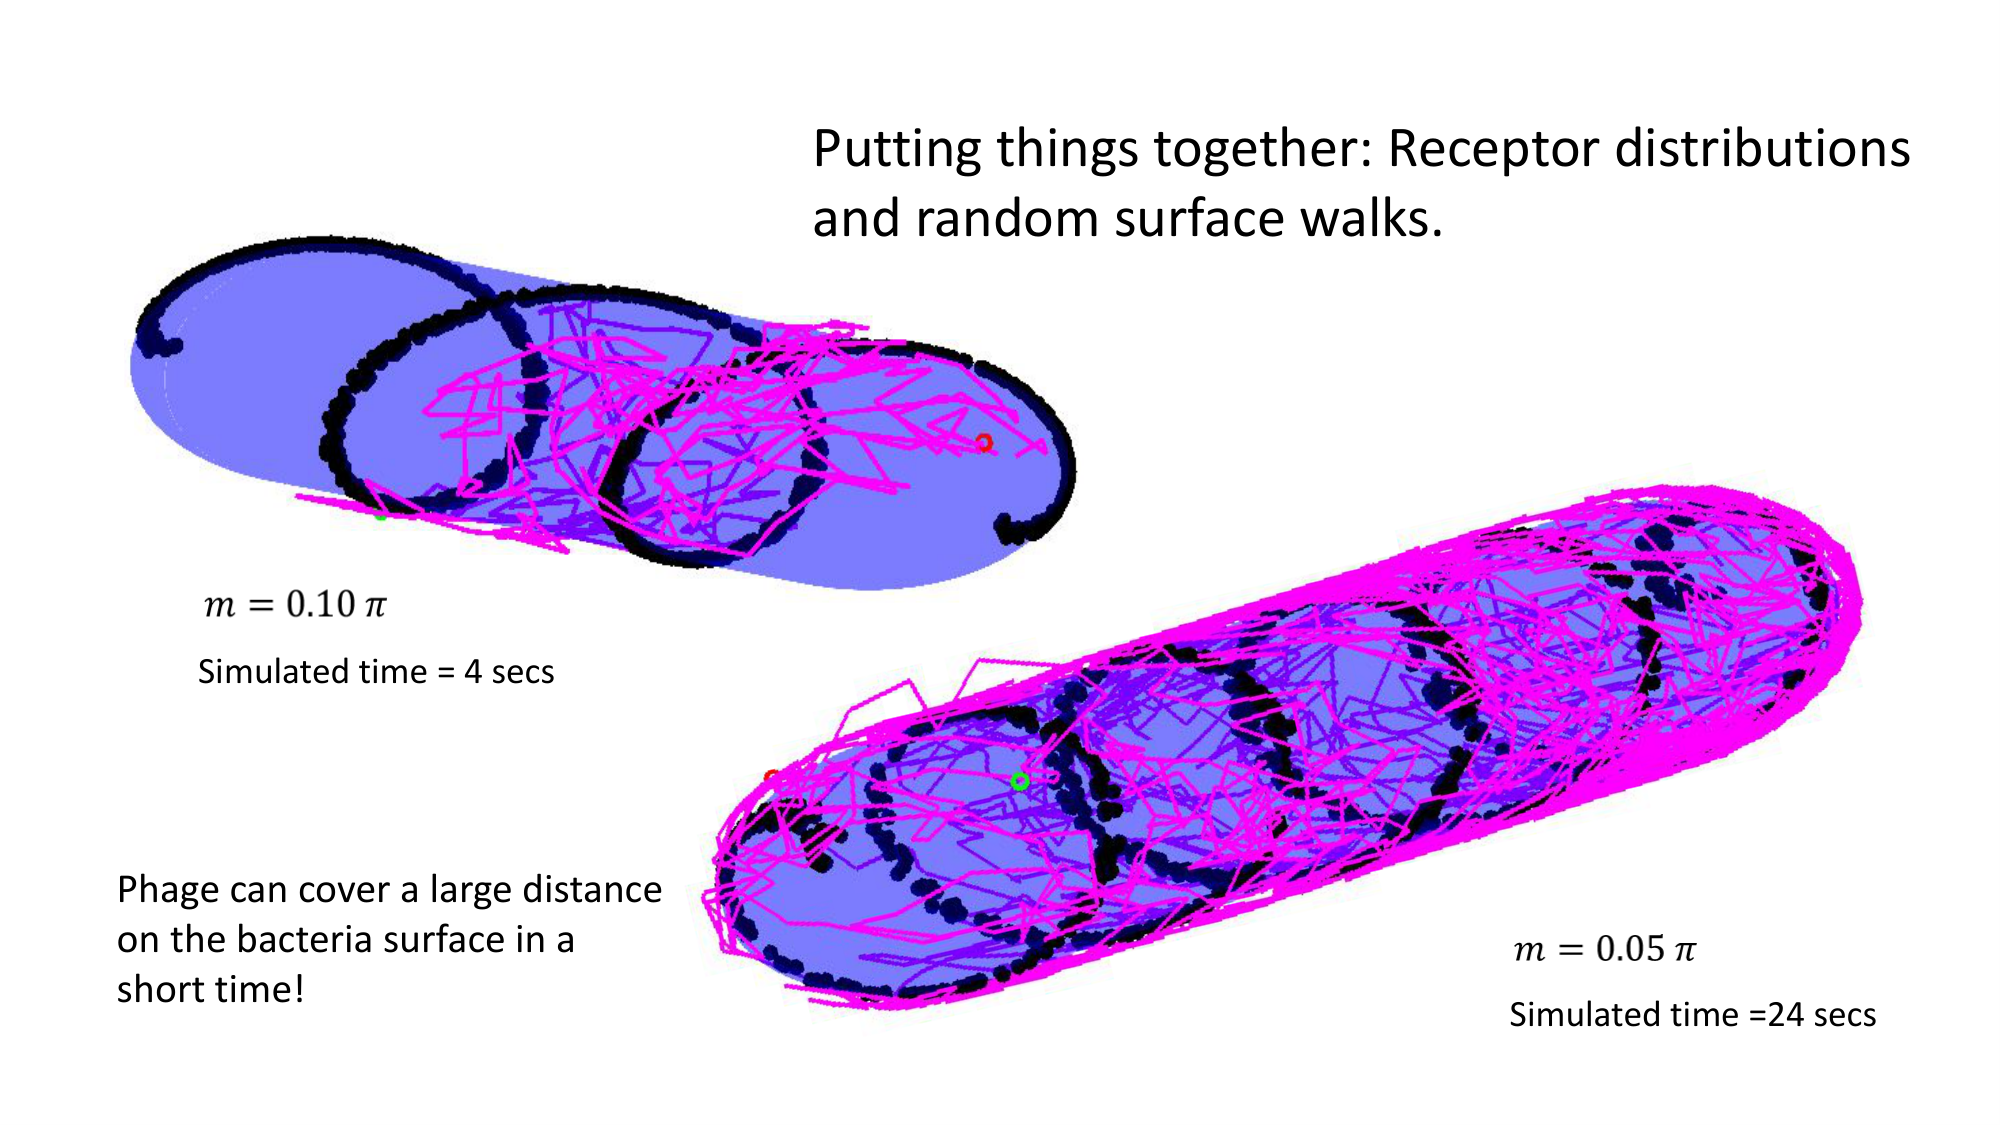
\includegraphics[width=0.48\linewidth]{slide_surface_walks.png}
\caption{Receptor model and surface search. (A, B) 1000 receptors in a helical band for pitch angles $m=0.01\pi$--$0.15\pi$: small $m$ gives a near-uniform coat, larger $m$ a helix. (C) Surface random walks of attached phage after 4\,s and 24\,s of simulated time; phage cover micrometres of the surface in seconds. \todo{Regenerate from \texttt{tiger.model.plotting}.}}
\label{fig:receptors}
\end{figure}

\begin{figure}[!ht]
\centering
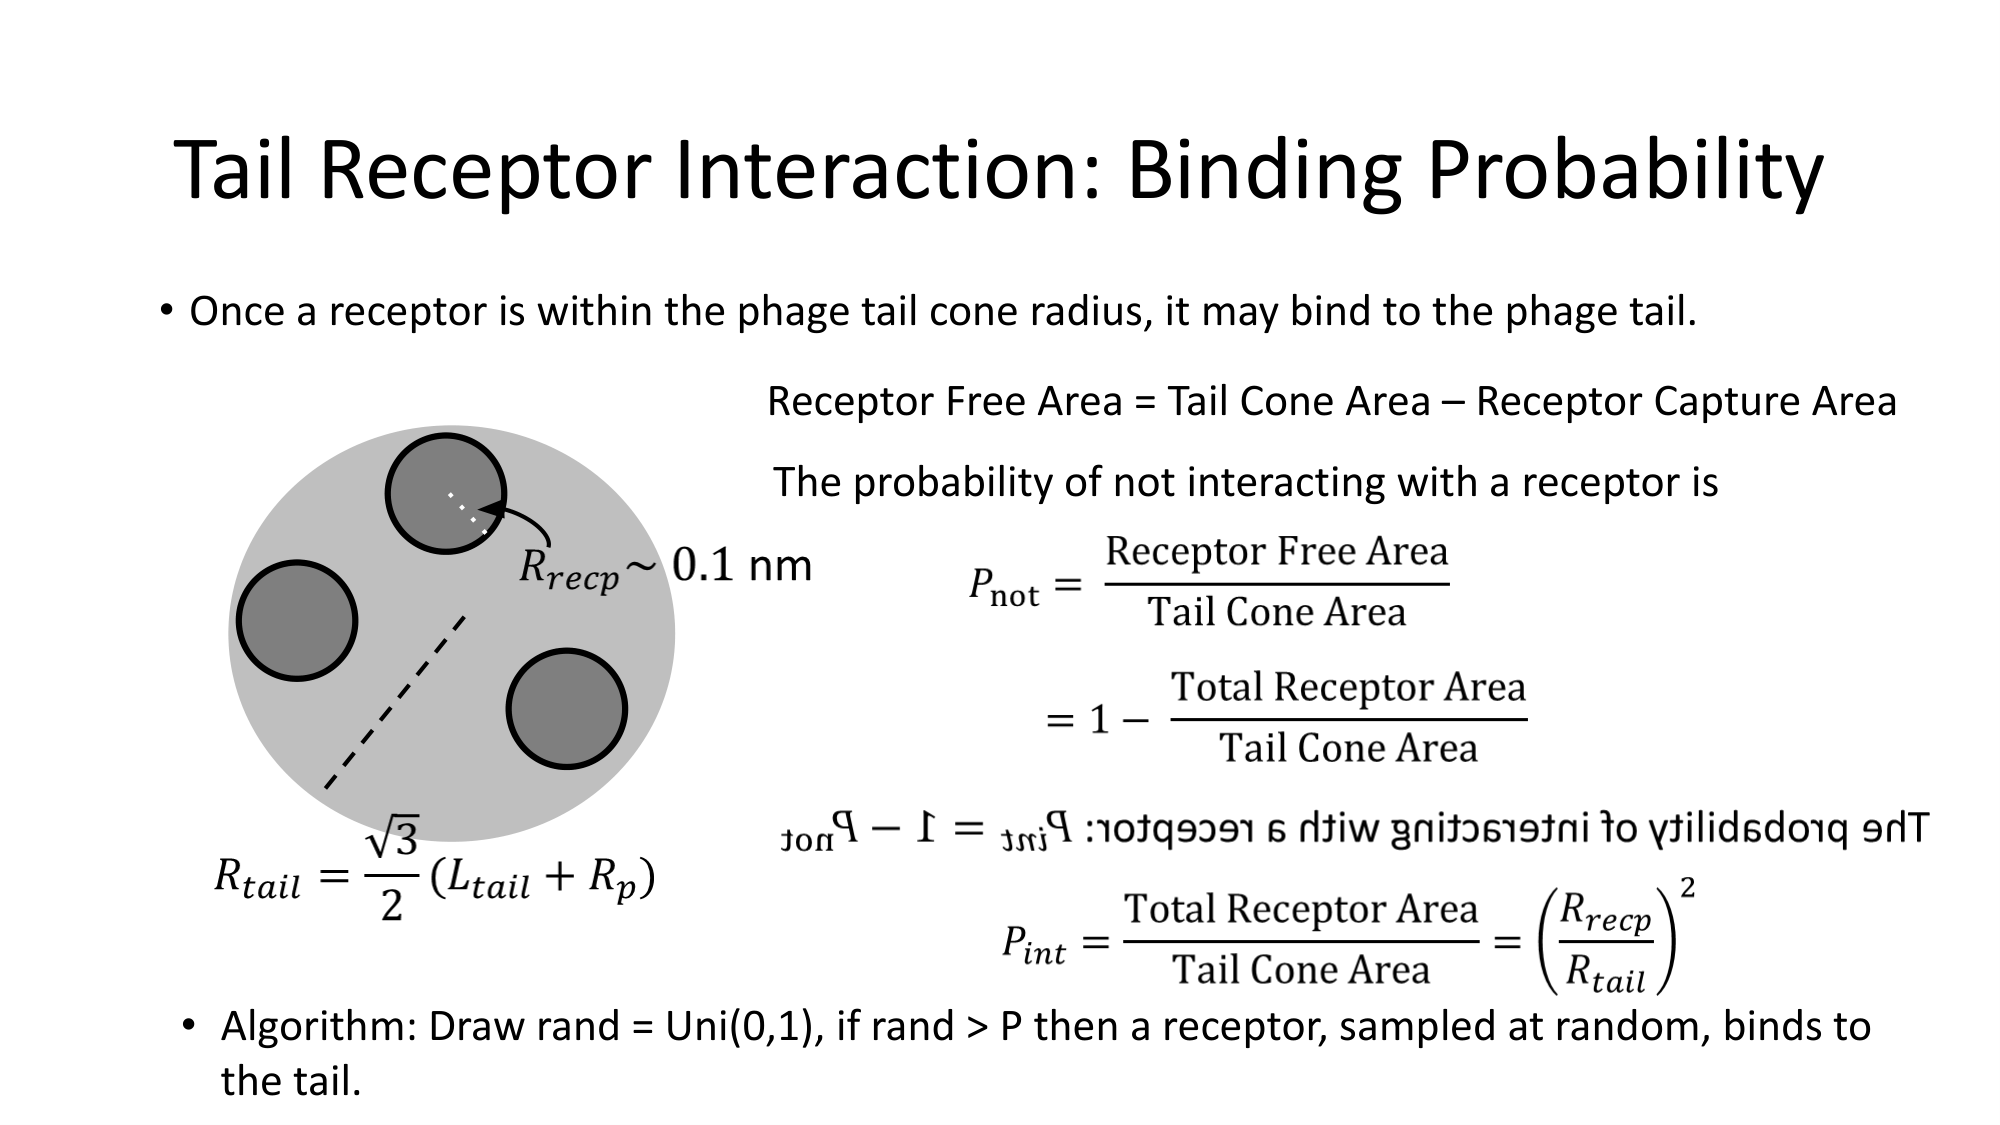
\includegraphics[width=0.48\linewidth]{slide_binding_probability.png}\hfill
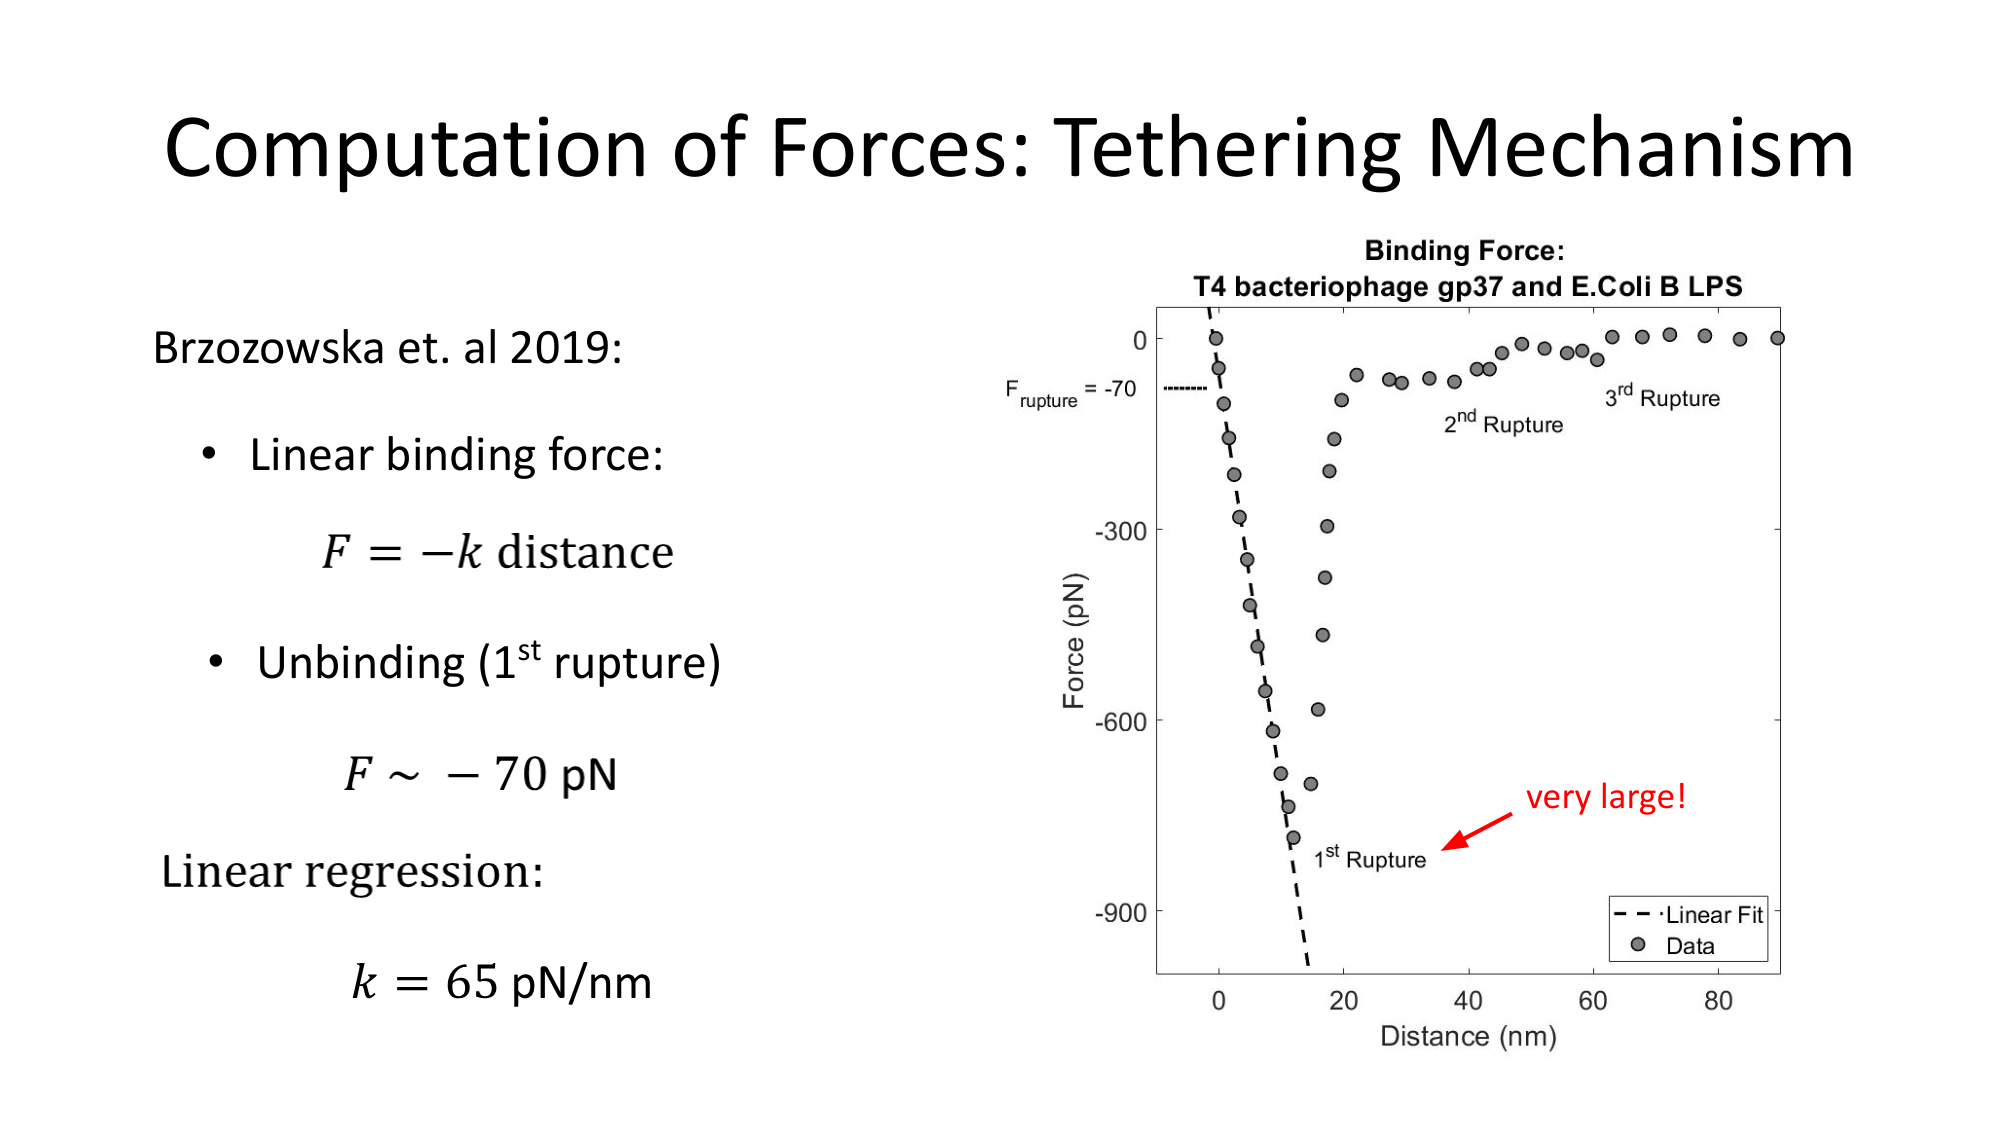
\includegraphics[width=0.48\linewidth]{slide_brzozowska_force.png}\\[4pt]
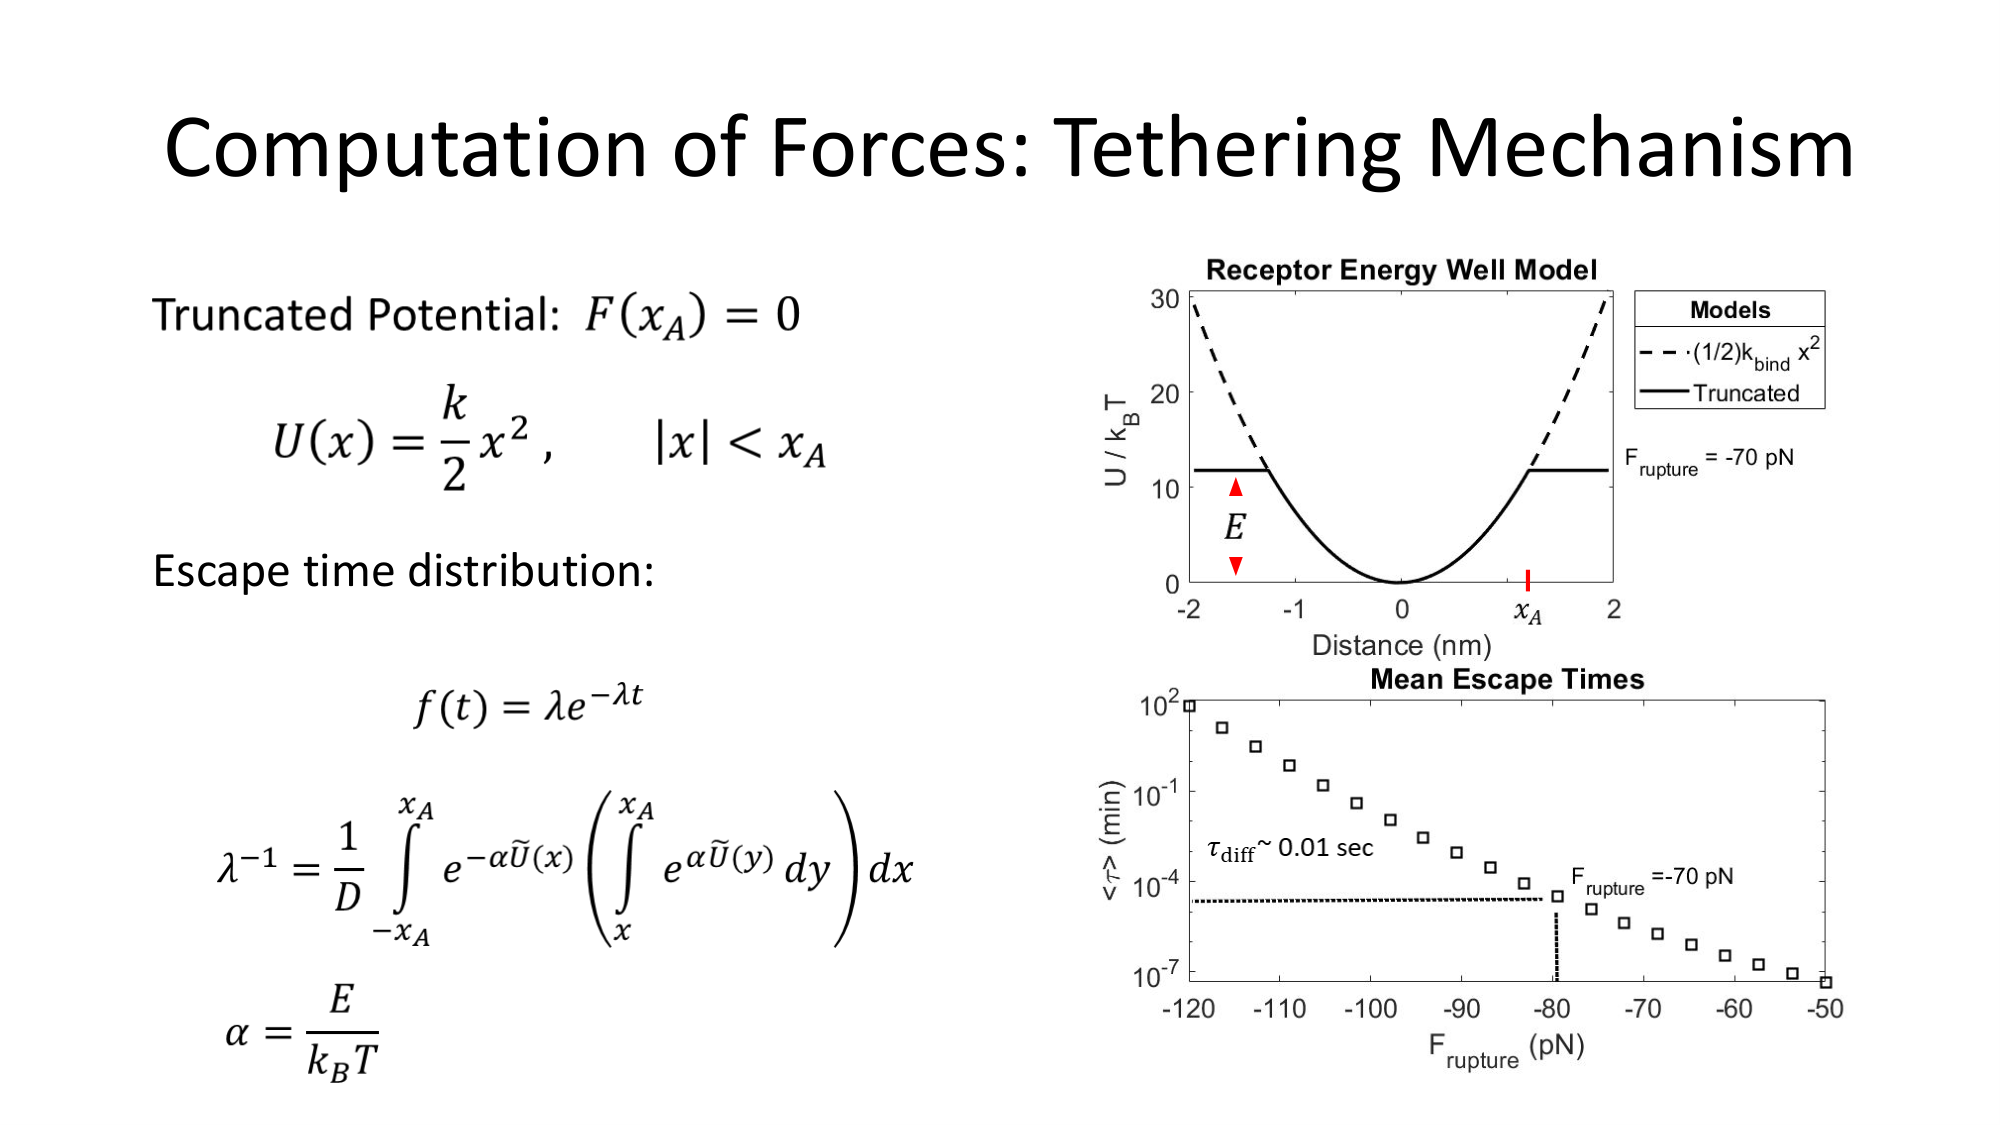
\includegraphics[width=0.6\linewidth]{slide_truncated_potential.png}
\caption{Tail--receptor binding, tether and bond lifetime. (A) Binding probability from the receptor-covered fraction of the tail cone. (B) gp37--LPS force--distance curve\cite{brzozowska2019} with linear fit $k_{\rm bind}=65$\,pN\,nm$^{-1}$ and first rupture near 70\,pN. (C) Truncated harmonic potential and mean escape time vs rupture force from Eq.~\eqref{eq:mfpt}. \todo{Regenerate with experiment E5.}}
\label{fig:force}
\end{figure}

\begin{figure}[!ht]
\centering
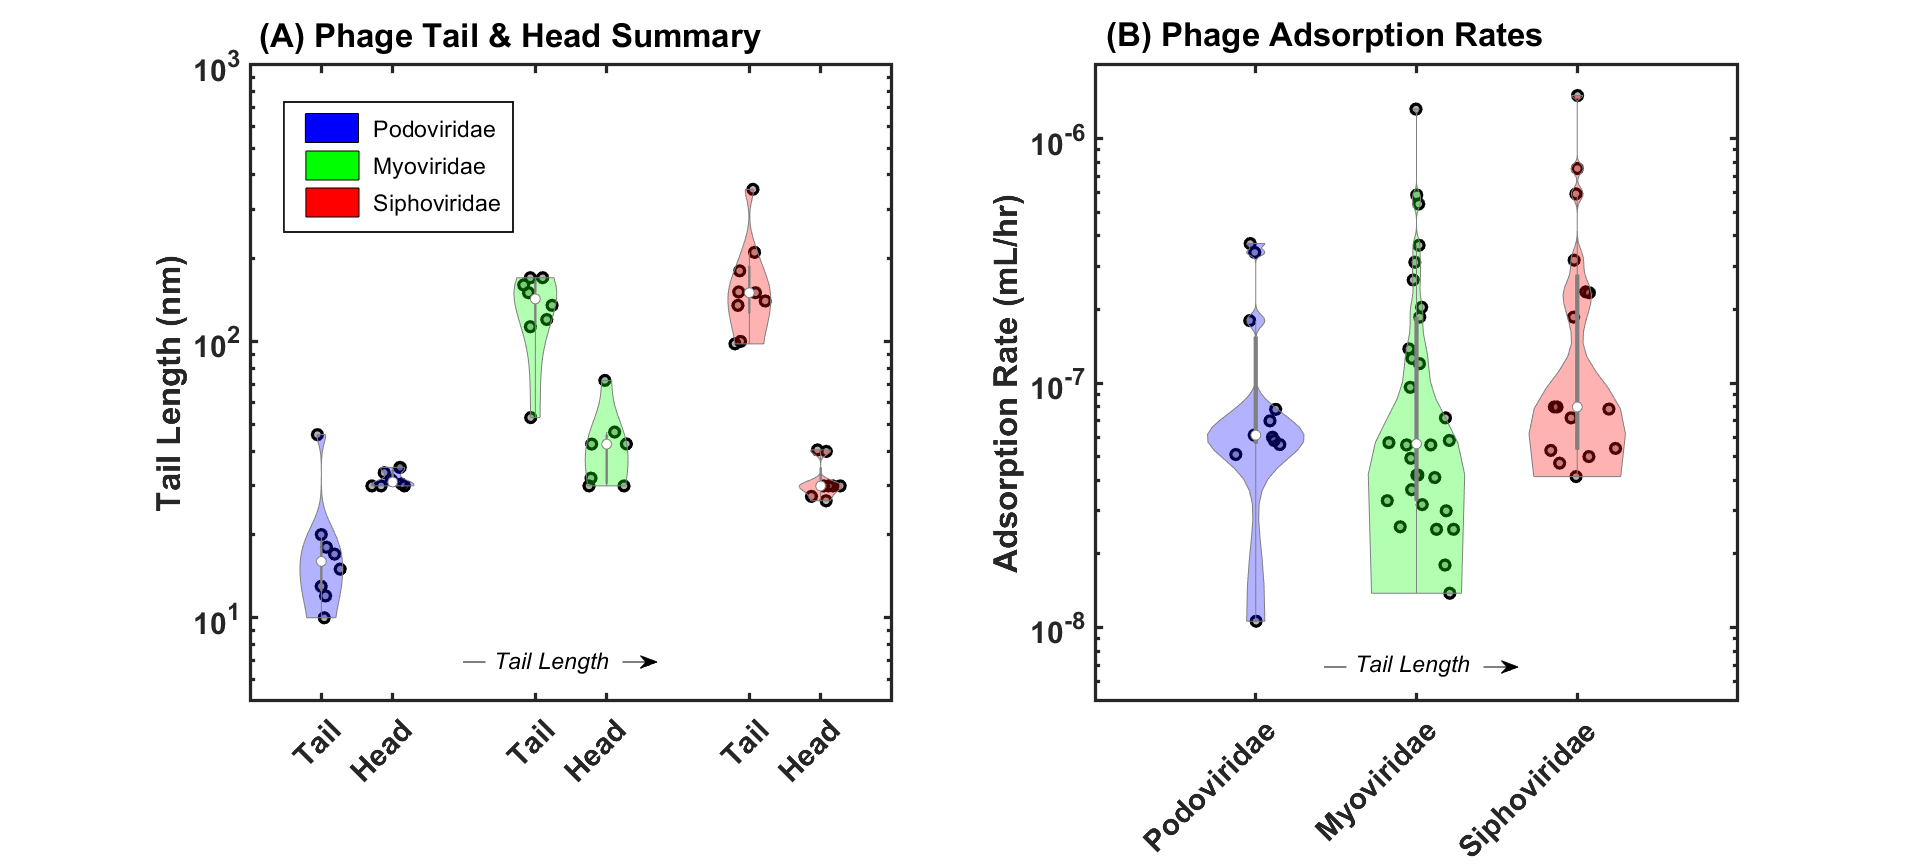
\includegraphics[width=\linewidth]{fig_adsorption_AB.png}\\
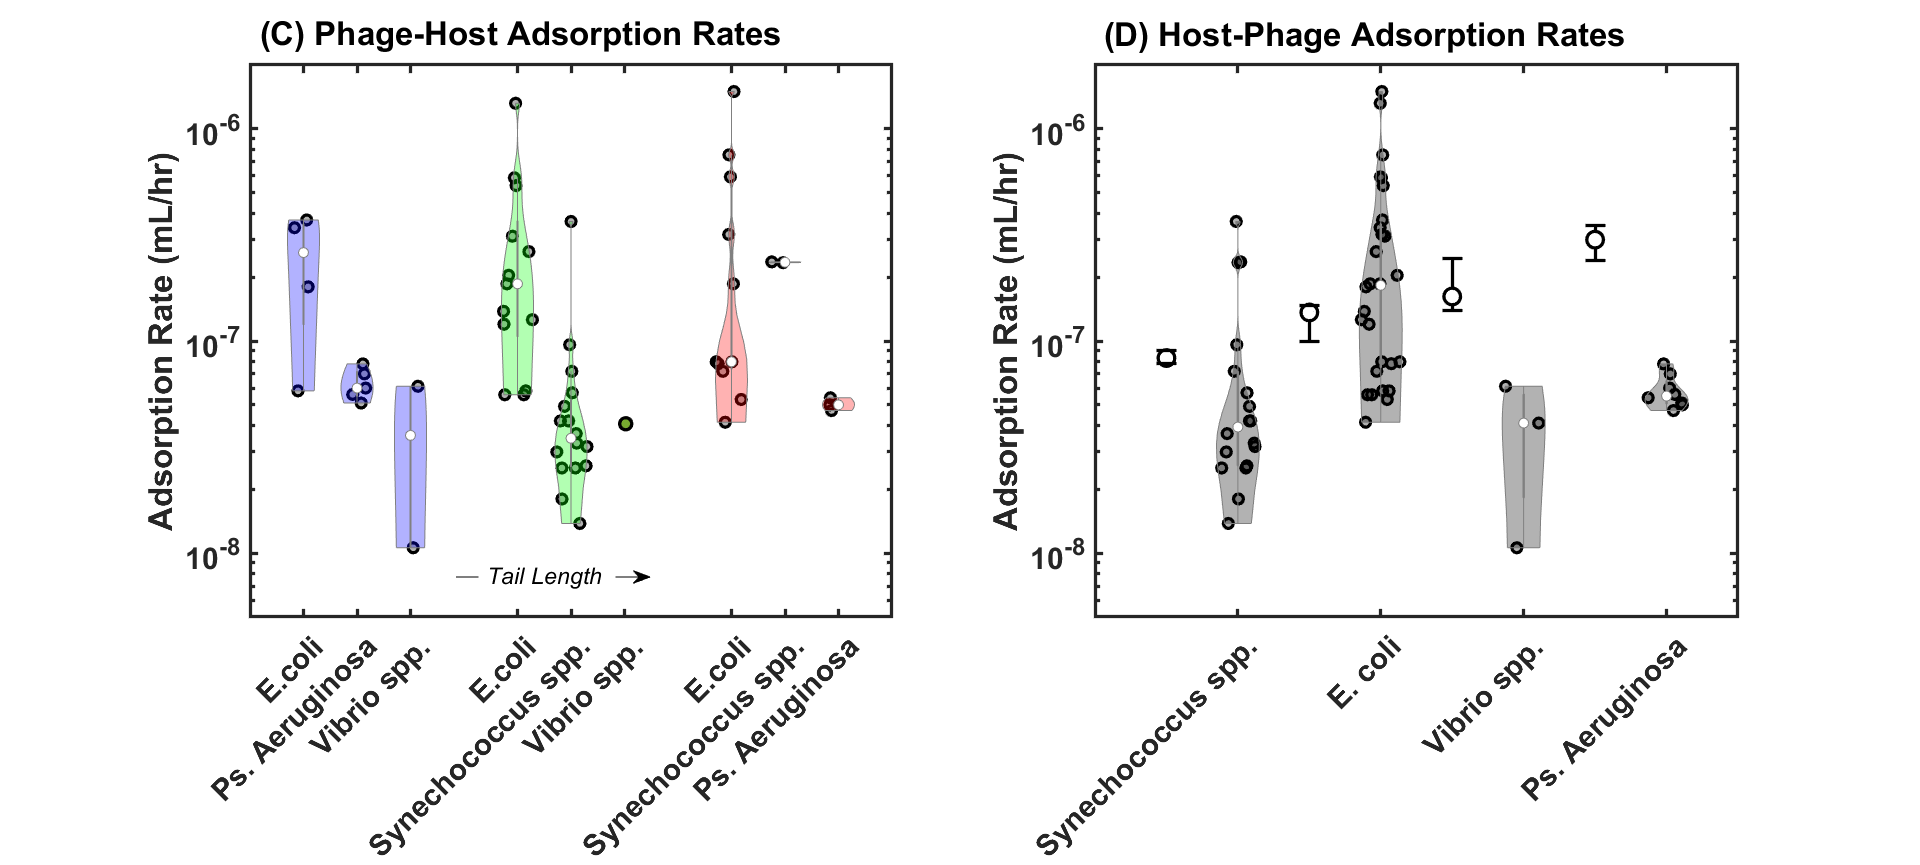
\includegraphics[width=\linewidth]{fig_adsorption_CD.png}
\caption{Literature adsorption survey (violin plots; white circles are medians, bars the interquartile range). (A) Tail length and capsid size by family. (B) Adsorption rate by family. (C) Adsorption rate by family and host. (D) Adsorption rate by host; open circles with bars are bootstrapped ballistic predictions $\pi R_C^2v_B$. \note{Figure from the earlier 57-measurement dataset; regenerate from \texttt{data/adsorption\_data.xlsx} with experiment E4.}}
\label{fig:adsorption}
\end{figure}

\begin{figure}[!ht]
\centering
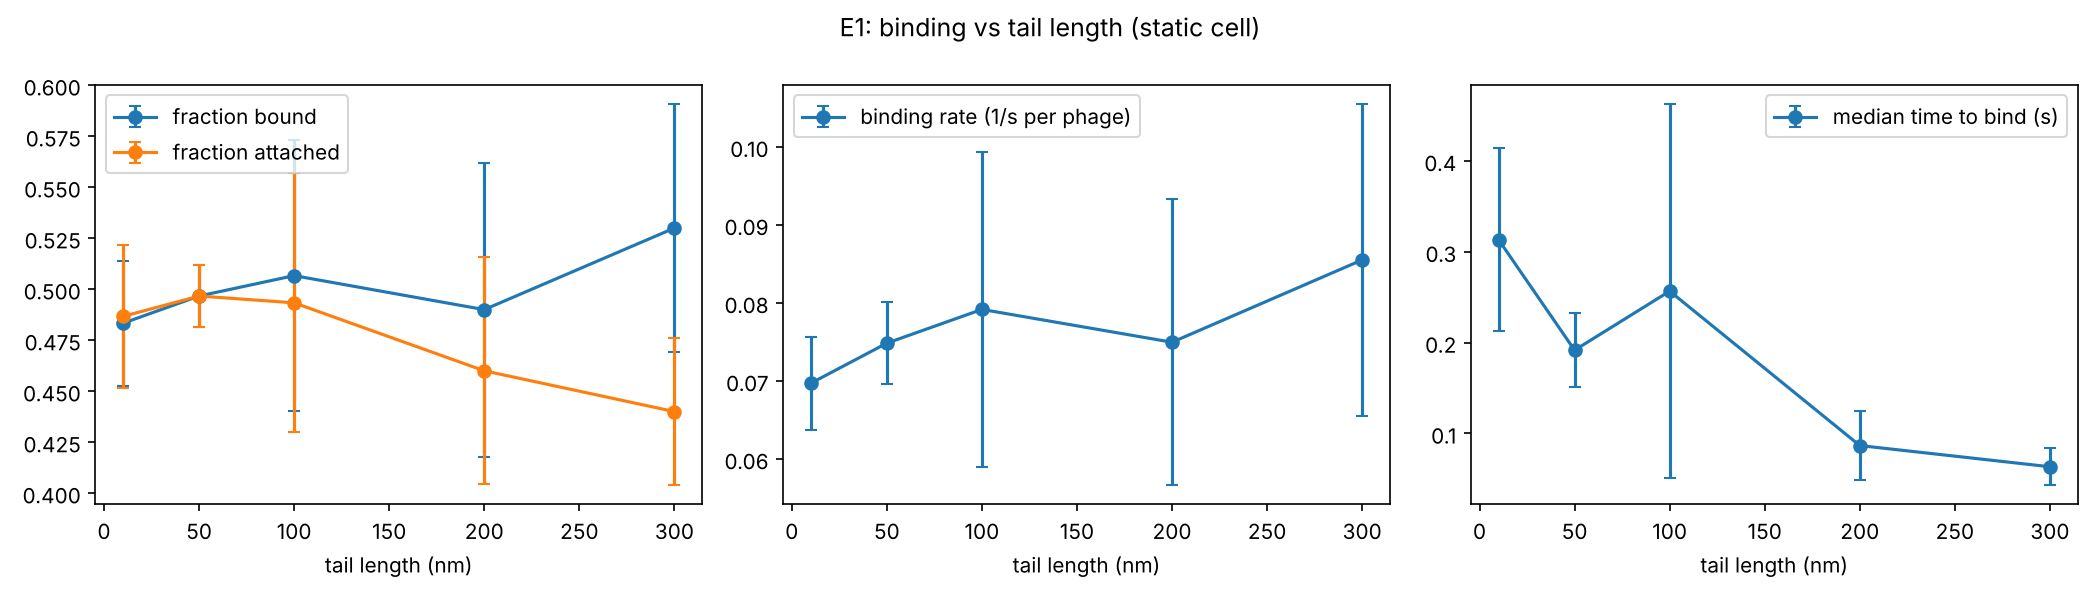
\includegraphics[width=0.49\linewidth]{prelim_E1_binding_vs_tail.png}\hfill
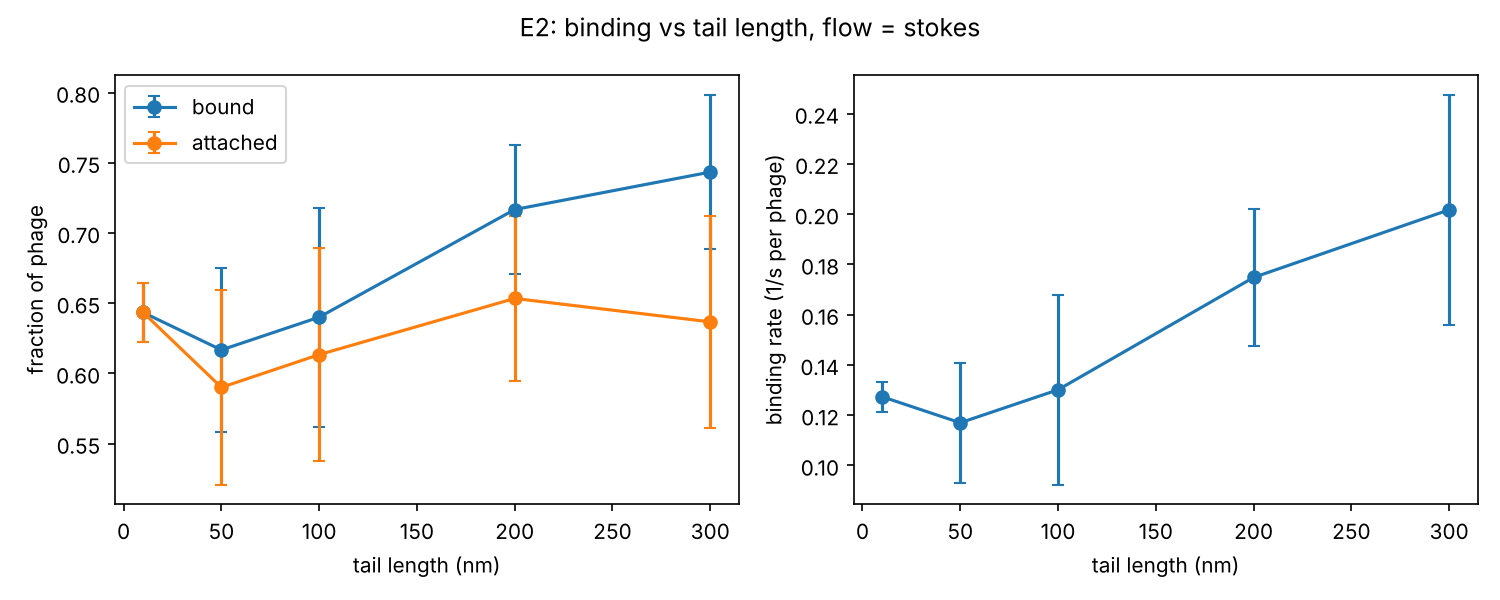
\includegraphics[width=0.49\linewidth]{prelim_E2_binding_vs_tail_stokes.png}\\
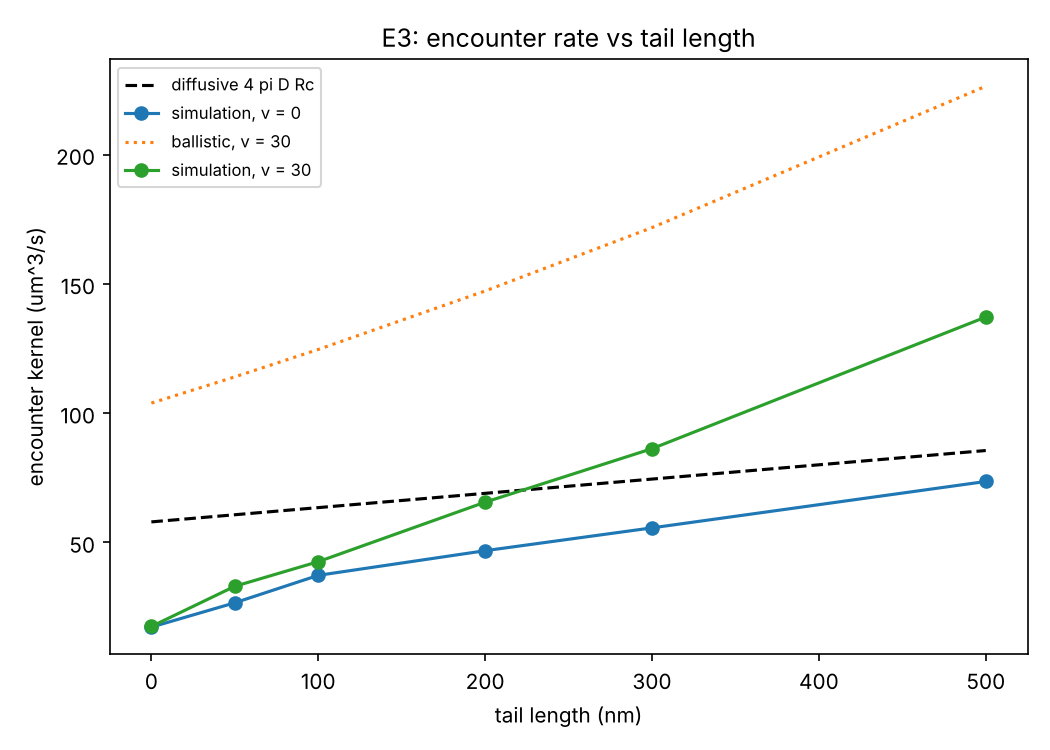
\includegraphics[width=0.55\linewidth]{prelim_E3_encounter_vs_tail.png}
\caption{\prelim{Preliminary} simulations. (A) E1, static cell: fraction attached and bound, binding rate and median time to bind vs tail length. (B) E2, cell swimming at 30\,$\mu$m\,s$^{-1}$ (Stokes flow). (C) E3, encounter kernel vs tail length: simulation (points) against the diffusive and ballistic limits. MATLAB binding rule, 100 phages, 12\,s, 3 replicates (A, B); 20{,}000 phages (C).}
\label{fig:prelim}
\end{figure}

\begin{table}[!ht]
\centering
\caption{Encounter-rate predictors per Study group (family $\times$ host) from \texttt{data}, computed by \texttt{tiger.analysis.kernel\_predictors}. \todo{Regenerate after host parameters are reconciled.}}
\label{tbl:predictors}
\small
\begin{tabular}{llrrrrr}
\toprule
Family & Host & $n$ & $R_C$ ($\mu$m) & $\beta_{\rm ball}$ & $\beta_{\rm diff}$ & median $k$ \\
 & & & & \multicolumn{3}{c}{(mL\,h$^{-1}$)}\\
\midrule
Sipho & Enterobacteriaceae & 10 & 0.85 & $2.5\times10^{-7}$ & $1.2\times10^{-5}$ & $8.0\times10^{-8}$\\
Sipho & Synechococcaceae & 2 & 0.88 & $1.3\times10^{-7}$ & --- & $2.4\times10^{-7}$\\
Sipho & Pseudomonadaceae & 4 & 0.77 & $5.0\times10^{-8}$ & $6.5\times10^{-7}$ & $5.4\times10^{-7}$\\
Myo & Synechococcaceae & 16 & 0.85 & $1.2\times10^{-7}$ & --- & $3.5\times10^{-8}$\\
Myo & Enterobacteriaceae & 14 & 0.82 & $2.3\times10^{-7}$ & $1.1\times10^{-5}$ & $1.9\times10^{-7}$\\
Myo & Vibrionaceae & 4 & 0.57 & $2.4\times10^{-7}$ & $3.8\times10^{-5}$ & $5.2\times10^{-8}$\\
Myo & Pseudomonadaceae & 2 & 0.79 & $5.3\times10^{-8}$ & $6.7\times10^{-7}$ & $4.6\times10^{-7}$\\
Podo & Pseudomonadaceae & 6 & 0.64 & $3.5\times10^{-8}$ & $5.5\times10^{-7}$ & $8.2\times10^{-7}$\\
Podo & Vibrionaceae & 2 & 0.46 & $1.6\times10^{-7}$ & $3.1\times10^{-5}$ & $3.5\times10^{-8}$\\
Podo & Enterobacteriaceae & 6 & 0.72 & $1.8\times10^{-7}$ & $9.8\times10^{-6}$ & $3.6\times10^{-7}$\\
\bottomrule
\end{tabular}
\end{table}

% =====================================================================
\clearpage
% supplement.tex -- included at the end of main.tex
\clearpage
\renewcommand{\thefigure}{S.\arabic{figure}}
\renewcommand{\thetable}{S.\arabic{table}}
\renewcommand{\theequation}{S.\arabic{equation}}
\setcounter{figure}{0}
\setcounter{table}{0}
\setcounter{equation}{0}

 {\LARGE \noindent \textbf{Supplementary Material}}

%=====================================================================
\subsection*{S1. Hydrodynamics}

\paragraph{S1.1 Navier--Stokes equations.} Mass conservation in a material volume $V(t)$ gives $\frac{d}{dt}\int_V\rho\,dV=0$. The Reynolds transport theorem turns this into the continuity equation
\begin{equation}
\frac{\partial\rho}{\partial t}+\nabla\cdot(\rho\bm u)=0 ,
\end{equation}
which reduces to $\nabla\cdot\bm u=0$ for an incompressible fluid. Momentum balance on the same volume, with surface stresses $\bm\sigma\cdot\hat{\bm n}$ and body force $\bm f$, gives Cauchy's equation
\begin{equation}
\rho\frac{D\bm u}{Dt}=\nabla\cdot\bm\sigma+\bm f .
\end{equation}
For a Newtonian fluid, $\bm\sigma=-p\bm I+\eta\left(\nabla\bm u+\nabla\bm u^{T}\right)$. With $\nabla\cdot\bm u=0$ this yields the incompressible Navier--Stokes equations.

Lengths are scaled by $a$, velocities by $U$ and pressure by $\eta U/a$. Then
\begin{equation}
\mathrm{Re}\left(\frac{\partial\bm u}{\partial t}+\bm u\cdot\nabla\bm u\right)=-\nabla p+\nabla^2\bm u+\bm f,\qquad \mathrm{Re}=\frac{\rho Ua}{\eta}.
\end{equation}
For \textit{E.~coli} ($a\approx1\,\mu$m, $U\approx30\,\mu$m\,s$^{-1}$, water), $\mathrm{Re}\approx3\times10^{-5}$. For a phage the value is smaller still. The inertial terms are therefore dropped, which gives the Stokes equations\cite{purcell1977life,happel1983}.

\paragraph{S1.2 Stokes flow past a translating sphere.} The sphere has radius $R$ and velocity $\bm v$, and the fluid is at rest at infinity. Linearity and isotropy restrict the solution to the form
\begin{equation}
\bm u(\bm r)=A(r)\,\bm v+B(r)\,\frac{\bm r(\bm v\cdot\bm r)}{r^2}.
\end{equation}
The general solution is a combination of a Stokeslet (decaying as $1/r$) and a source dipole (decaying as $1/r^3$),
\begin{equation}
\bm u=A_1\left(\frac{\bm v}{r}+\frac{\bm r(\bm v\cdot\bm r)}{r^3}\right)+A_2\left(\frac{\bm v}{r^3}-\frac{3\bm r(\bm v\cdot\bm r)}{r^5}\right).
\end{equation}
No slip, $\bm u(|\bm r|=R)=\bm v$ for every direction $\hat{\bm r}$, gives two conditions:
\begin{equation}
\frac{A_1}{R}+\frac{A_2}{R^3}=1,\qquad \frac{A_1}{R}-\frac{3A_2}{R^3}=0
\quad\Longrightarrow\quad A_1=\frac{3R}{4},\quad A_2=\frac{R^3}{4}.
\end{equation}
Substitution recovers Eq.~\eqref{eq:stokes_sphere}. The drag follows from the Stokeslet strength, $\bm F=-8\pi\eta A_1\bm v=-6\pi\eta R\bm v$. This is the drag used for the phage friction coefficient $\gamma=6\pi\eta R_P$.

\paragraph{S1.3 Rotating sphere and the inertial correction (remark).} A sphere rotating at $\bm\omega$ generates the rotlet flow $\bm u_0=R^3\bm\omega\times\bm r/r^3$. The disturbance pressure is identically zero. One of the source notes adds the first inertial correction, a secondary flow $\bm u_1$ that draws fluid in at the poles and pushes it out at the equator. This $\bm u_1$ was proposed as a ``non-laminar vortex'' that could attract phage toward the cell.

\note{This correction scales as $\mathrm{Re}_\omega=\rho\omega R^2/\eta$ relative to $\bm u_0$. For the cell body, $\omega\sim 10$--$20$\,rad\,s$^{-1}$ and $R\sim1\,\mu$m give $\mathrm{Re}_\omega\sim10^{-5}$. For the flagellar bundle ($\omega\sim 600$\,rad\,s$^{-1}$, $R\sim 10$\,nm) it is smaller still. The secondary flow cannot produce a measurable attraction, so it is omitted from the model. The point is kept here because it appears in earlier drafts.}

%=====================================================================
\subsection*{S2. Phage--receptor first-passage times}
Consider independent particles in a deep potential well $U(x)$. They are initially inside the well and slowly leak out across the barrier. The overdamped Langevin equation $\gamma\dot x=-U'(x)+\eta(t)$ produces probability densities $P(x,t)$ that obey the Fokker--Planck (Smoluchowski) equation
\begin{equation}
\frac{\partial P}{\partial t}=\frac{\partial}{\partial x}\left(\frac{U'}{\gamma}P\right)+D\frac{\partial^2P}{\partial x^2}
= D\frac{\partial}{\partial x}\left[e^{-\tilde U}\frac{\partial}{\partial x}\left(e^{\tilde U}P\right)\right],\qquad \tilde U=\frac{U}{k_BT},
\end{equation}
where we used the Stokes--Einstein relation $\gamma D=k_BT$. The initial condition is $P(x,0)=\delta(x-x_0)$. Absorbing boundaries $P(\pm x_A,t)=0$ remove trajectories at their first exit.

\paragraph{Survival and first-passage density.} The survival probability is $S(t)=\int_{-x_A}^{x_A}P\,dx=\mathrm{Prob}(\tau\ge t)$. The first-passage density is then
\begin{equation}
f(t)=-S'(t)=-\int\frac{\partial P}{\partial t}\,dx .
\end{equation}

\paragraph{Characteristic function.} Define $\varphi(\omega)=E[e^{i\omega\tau}]=\int_0^\infty e^{i\omega\tau}f(\tau)\,d\tau$. Integrating by parts in time, with $P\to0$ as $t\to\infty$ and $\int P(x,0)\,dx=1$, gives
\begin{equation}
\varphi(\omega)=1+i\omega\int g(x,\omega)\,dx,\qquad g(x,\omega)=\int_0^\infty e^{i\omega\tau}P(x,\tau)\,d\tau .
\end{equation}
Transforming the Fokker--Planck equation in the same way gives an ordinary differential equation for $g$,
\begin{equation}
D\frac{d}{dx}\left[e^{-\tilde U}\frac{d}{dx}\left(e^{\tilde U}g\right)\right]=-\delta(x-x_0)-i\omega g .
\end{equation}
For a deep well, the time to equilibrate inside the well is short compared with the escape time. To leading order in $\omega$ the flux through the barrier is then uniform. Integrating twice, with $g(\pm x_A)=0$, gives
\begin{equation}
\int g\,dx\simeq \varphi(\omega)\,\frac{1}{D}\int_{-x_A}^{x_A}e^{-\tilde U(x)}\int_x^{x_A}e^{\tilde U(y)}\,dy\,dx \equiv \frac{\varphi(\omega)}{\lambda}.
\end{equation}
Substituting this into the expression for $\varphi$ gives
\begin{equation}
\varphi(\omega)=\frac{\lambda}{\lambda-i\omega}\quad\Longrightarrow\quad f(t)=\lambda e^{-\lambda t},\qquad
\lambda^{-1}=\frac{1}{D}\int_{-x_A}^{x_A}e^{-\tilde U(x)}\int_x^{x_A}e^{\tilde U(y)}\,dy\,dx .
\end{equation}
The mean bond lifetime is $\langle t\rangle=\lambda^{-1}$. This is the Kramers result\cite{kramers1940brownian,zwanzig2001nonequilibrium} used in the main text. Under an applied load $F$ the potential is tilted, $\tilde U\to\tilde U-Fx/k_BT$, which produces the force dependence shown in the main-text bond-lifetime figure.

\note{The original note writes the characteristic function with both $s$ and $\omega$, and calls $g$ ``$i\omega$ times the Laplace transform''. Here $g$ is the transform itself (with $s=-i\omega$). The note also states the boundary condition $\partial_x(e^{\tilde U}g)|_0=0$ without justification. This holds only for a symmetric well with $x_0=0$. For general $x_0$ the double integral starts at $x_0$, and the deep-well result above holds to leading order.}

%=====================================================================
\subsection*{S3. Tether integration: RATTLE and Lennard-Jones}
\paragraph{Stiffness.} With $k_{\rm bind}=65$\,pN\,nm$^{-1}$ and $\gamma=6\pi\eta R_P\approx 2\times10^{-9}$\,kg\,s$^{-1}$, the tether relaxes in $\gamma/k_{\rm bind}\approx3\times10^{-8}$\,s. This is roughly five orders of magnitude below the Brownian step $\Delta t=10^{-2}$\,s. An explicit Euler step is therefore unstable. Two options are implemented:
\begin{enumerate}
\item the exact exponential update of the main text (tether section), which treats the tether analytically over each step;
\item treating the tether as a rigid constraint $|\bm p|\le L_{\rm tail}+R_P$ and enforcing it with RATTLE\cite{andersen1983rattle}.
\end{enumerate}

\paragraph{RATTLE.} For a holonomic constraint $\sigma(\bm x)=|\bm x-\bm x_r|^2-R^2=0$, each step does the following:
\begin{enumerate}
\item take an unconstrained step $\bm x^\star$;
\item find a Lagrange multiplier $\lambda$ such that $\sigma(\bm x^\star-\lambda\nabla\sigma(\bm x_{n}))=0$, by solving a scalar quadratic;
\item remove the velocity component along the constraint normal.
\end{enumerate}
In the overdamped limit only the position projection is needed. This is the same closest-point projection used for the surface walk (main-text surface-search projection).

\paragraph{Lennard-Jones contact.} Earlier MATLAB versions also included a truncated and shifted Lennard-Jones repulsion between the capsid and the cell wall,
\begin{equation}
U_{\rm LJ}(r)=4\epsilon\left[\left(\frac{\sigma}{r}\right)^{12}-\left(\frac{\sigma}{r}\right)^{6}\right]+\epsilon,\qquad r<2^{1/6}\sigma ,
\end{equation}
which is zero beyond $r=2^{1/6}\sigma$. The event-driven specular reflection (main text, event-driven collisions) replaces this term in the current code. The two give the same hard-core exclusion, but the reflection needs no small time step.

%=====================================================================
\subsection*{S4. Continuous-time random walk and capture times}
To model subdiffusive phage in mucus, the waiting time between jumps is drawn from a Mittag-Leffler-like power law with exponent $0<\alpha<1$\cite{metzler2000random,joiner2019impact}:
\begin{equation}
\tau=\Delta t\left(\frac{1}{U\,\Gamma(1-\alpha)}\right)^{1/\alpha},\qquad U\sim\mathrm U(0,1).
\end{equation}
The Python port uses the equivalent Pareto form $\tau=t_{\min}U^{-1/\alpha}$. The mean squared displacement grows as $\langle x^2\rangle=2dD_\alpha t^\alpha/\Gamma(1+\alpha)$.

The generalized diffusivity is calibrated so that the subdiffusive and normal walks give the same MSD at the observation time $t_{\rm obs}$:
\begin{equation}
D_\alpha=D_0\,\Gamma(1+\alpha)\,t_{\rm obs}^{1-\alpha}.
\end{equation}

The mean capture time of a phage starting at distance $r_0$ from a perfectly absorbing sphere of radius $R_C$ is finite only inside a bounded domain of radius $R_{\rm out}$. With a reflecting outer wall it is
\begin{equation}
\langle T\rangle=\frac{1}{6D}\left[\frac{2R_{\rm out}^3}{R_C}-\frac{2R_{\rm out}^3}{r_0}+R_C^2-r_0^2\right]\quad(\alpha=1).
\end{equation}
For $\alpha<1$ the mean diverges, and medians are reported instead\cite{joiner2019impact}. In the present study $\alpha=1$.

%=====================================================================
\subsection*{S5. Rest-frame rotation after a tumble}
When the cell tumbles, its new run direction $\hat{\bm v}=(v_x,v_y,v_z)$ is rotated back onto the body axis $\hat{\bm e}_x$, and the same rotation is applied to every phage position. With yaw $\psi=-\operatorname{atan2}(v_y,v_x)$ and pitch $\alpha=\arcsin v_z$,
\begin{equation}
\bm R=\bm R_y(\alpha)\,\bm R_z(\psi),\quad
\bm R_z(\psi)=\begin{pmatrix}\cos\psi&-\sin\psi&0\\ \sin\psi&\cos\psi&0\\0&0&1\end{pmatrix},\quad
\bm R_y(\alpha)=\begin{pmatrix}\cos\alpha&0&\sin\alpha\\0&1&0\\-\sin\alpha&0&\cos\alpha\end{pmatrix},
\end{equation}
so that $\bm R\hat{\bm v}=\hat{\bm e}_x$. The new direction is drawn from the run--tumble angle distribution, with mean turning angle $\approx68^\circ$\cite{berg2004coli}.

\note{The MATLAB uses \texttt{atan} rather than \texttt{atan2}, which flips the yaw for $v_x<0$. The Python port uses \texttt{arctan2}.}

%=====================================================================
\subsection*{S6. The encounter estimator is independent of concentration}
In a volume $V$ with $N_{\rm act}$ actively tracked phage, the encounter rate per cell is $\dot N_{\rm enc}=\beta\,c$ with $c=N_{\rm act}/V$. Over a window $\Delta t$ this gives
\begin{equation}
\beta=\frac{N_{\rm enc}\,V}{N_{\rm act}\,\Delta t}.
\end{equation}
Phages are independent and do not interact with each other. $N_{\rm enc}$ is therefore a sum of $N_{\rm act}$ independent Bernoulli trials with success probability $p=\beta\Delta t/V$. Its expectation is proportional to $N_{\rm act}$, so the estimator is unbiased for any phage concentration. Its relative error falls as $(N_{\rm act}p)^{-1/2}$.

Encountered phage are reinserted at the domain boundary, which keeps $N_{\rm act}$ fixed. The domain must be large enough ($R_{\rm out}\gtrsim 10R_C$) for the boundary depletion layer to be negligible. \todo{Check that the estimator reproduces $\beta_{\rm diff}$ for a non-motile cell; the preliminary E3 runs undercount because the capture shell is thin.}

%=====================================================================
\subsection*{S7. Material from the notes not used in this study}

\paragraph{Multigrid solvers.} The notes contain a geometric multigrid V-cycle for the 1-D Poisson problem (Fig.~\ref{fig:S_multigrid}): Gauss--Seidel smoothing, full-weighting restriction and linear prolongation, which converges in $O(N)$ work. None of the main-text methods needs an elliptic solver:
\begin{itemize}
\item the LBM is explicit;
\item the Brownian dynamics is Lagrangian;
\item the Kramers integrals are one-dimensional quadratures.
\end{itemize}
Multigrid would be useful only as an optional independent check of the encounter kernel. In that check, the steady advection--diffusion equation
\begin{equation}
\bm u\cdot\nabla c=D_P\nabla^2 c,\qquad c|_{\partial\Omega_C}=0,\quad c\to c_\infty ,
\end{equation}
is solved in the rest frame of the cell, using the Stokes or LBM flow $\bm u$. The kernel is then the total flux, $\beta=\frac{D_P}{c_\infty}\oint\nabla c\cdot\hat{\bm n}\,dS$. This would test the Brownian-dynamics estimate of $\beta$ against a deterministic solution at high P\'eclet number, where the thin boundary layer makes Brownian dynamics noisy. \todo{Decide whether this cross-check is worth implementing; a 3-D multigrid or an off-the-shelf sparse solver would both work.}

\begin{figure}[!ht]
\centering
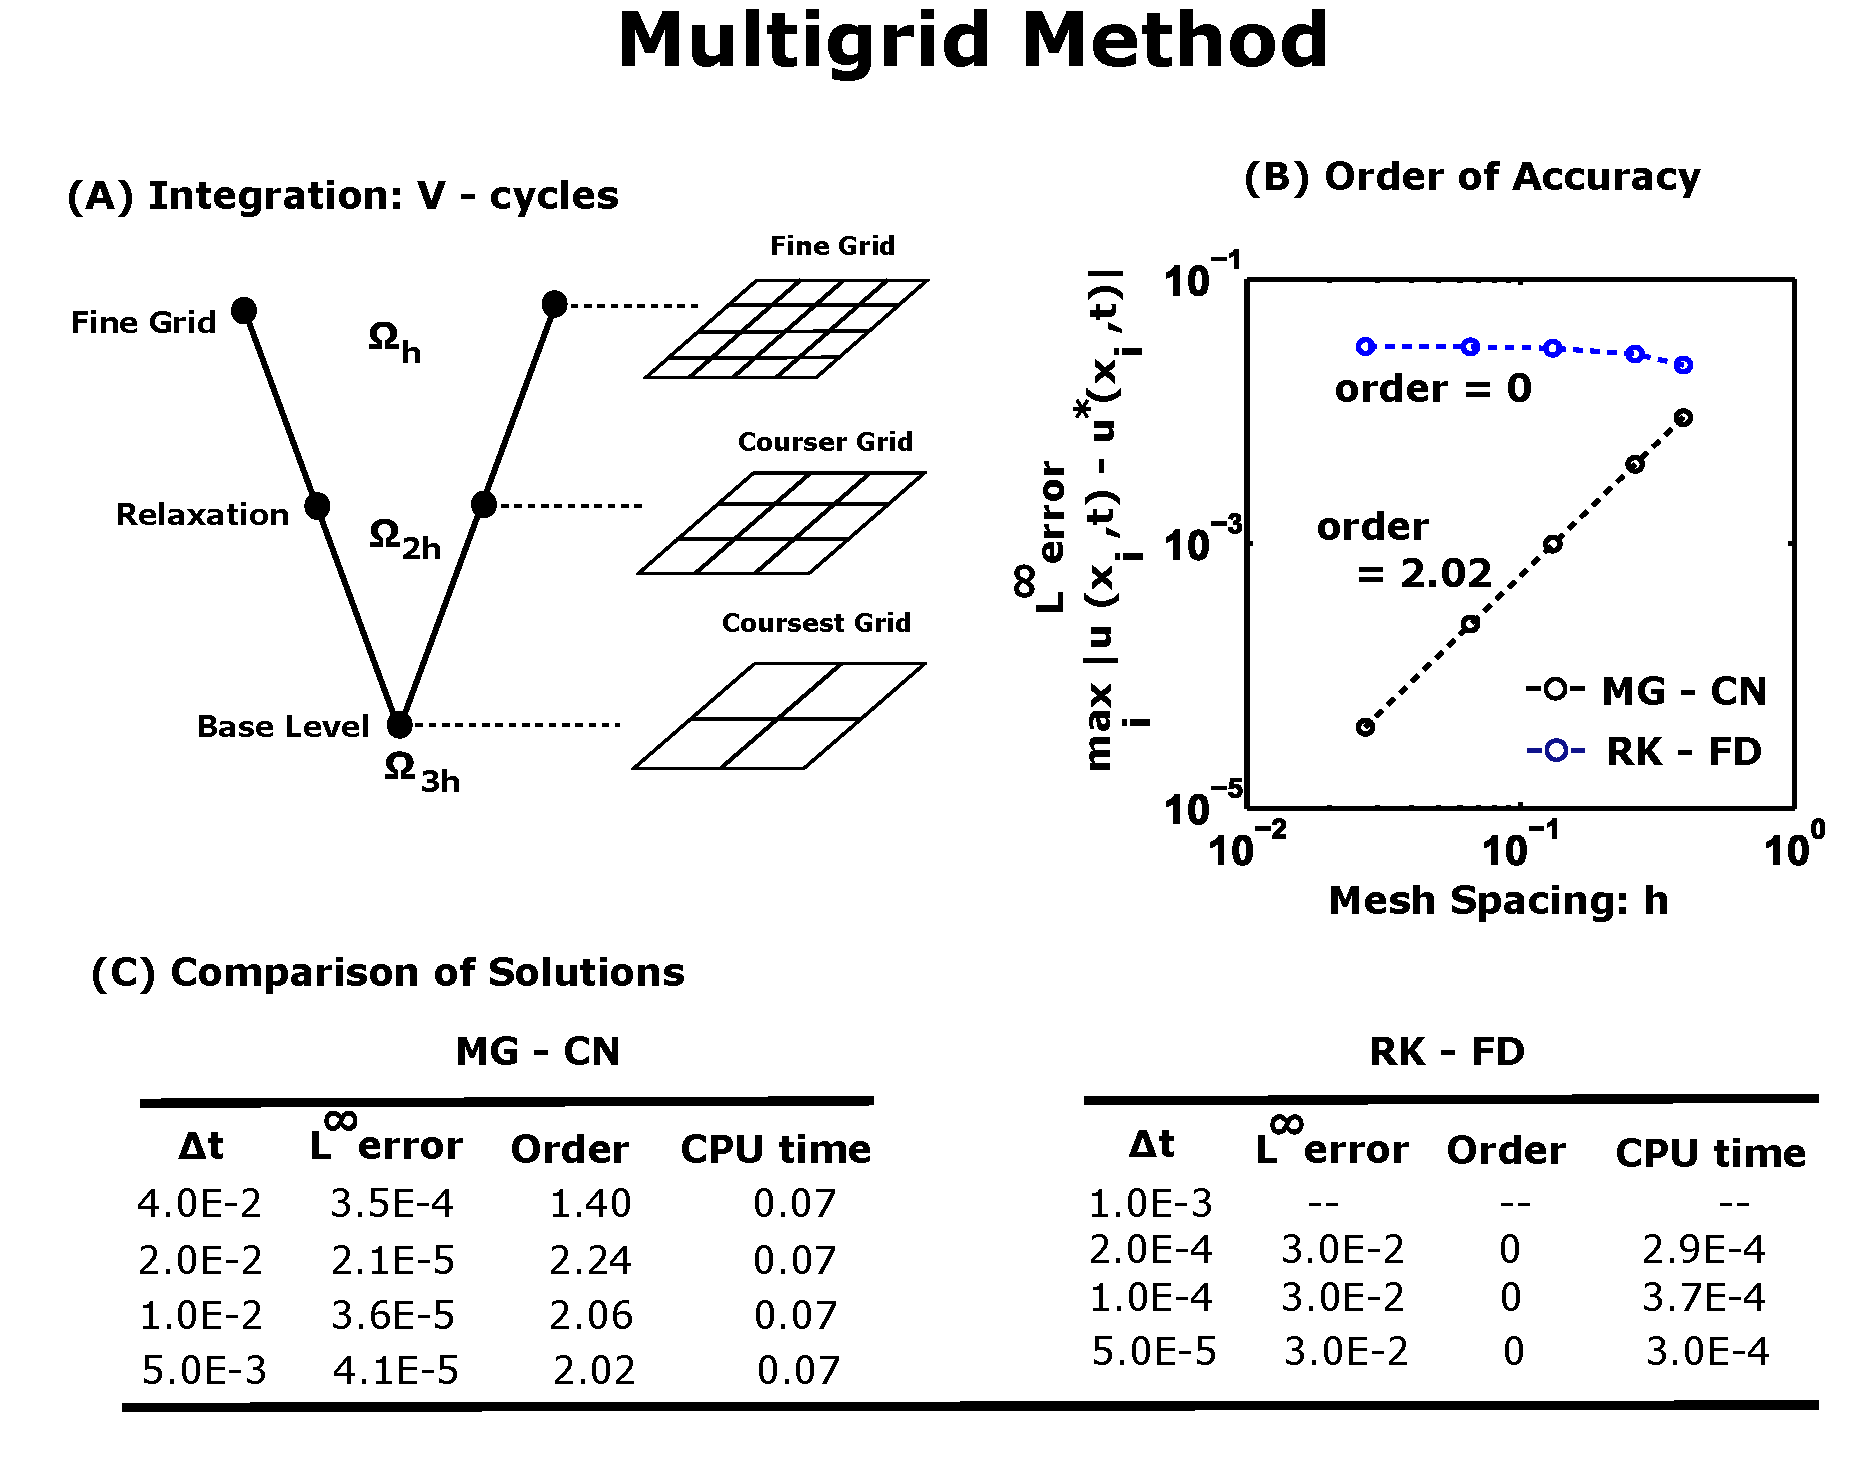
\includegraphics[width=0.6\textwidth]{Multigrid_1D_Results.pdf}
\caption{1-D multigrid V-cycle results from the notes (not used in the main text).}
\label{fig:S_multigrid}
\end{figure}

\paragraph{Population-level agent-based model.} The bacterium--phage life-cycle model (Fig.~\ref{fig:S_abm}) tracks infection, latent period, burst and lysis across a population. This sits one level above the single-cell question studied here. The encounter and binding rates computed in this work are the inputs such a model needs, so it is a natural follow-up, but it is not part of this manuscript.

\begin{figure}[!ht]
\centering
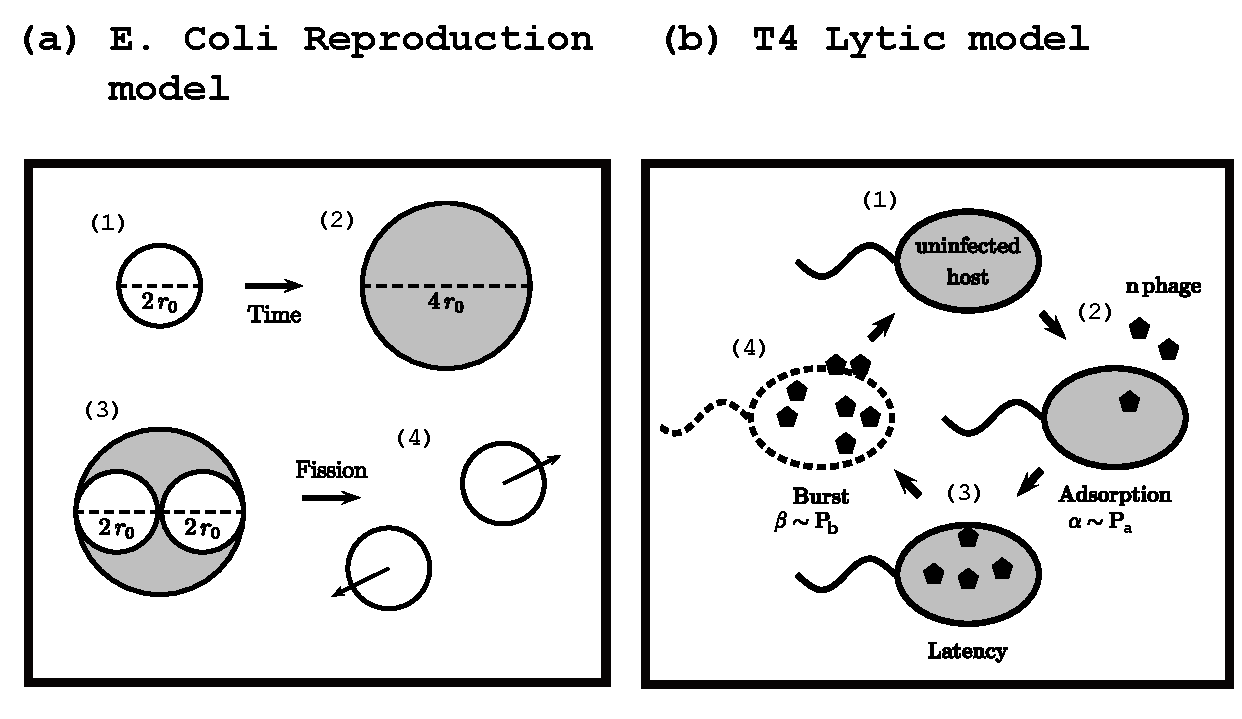
\includegraphics[width=0.45\textwidth]{bac_phage_life.pdf}\hfill
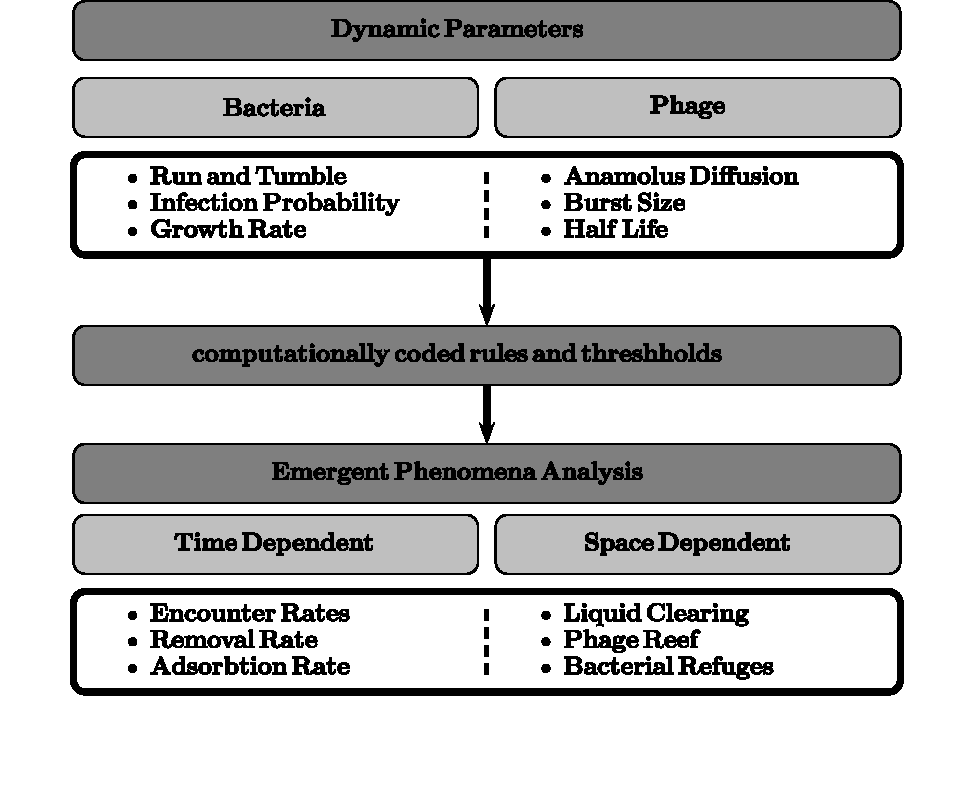
\includegraphics[width=0.45\textwidth]{ABM2.pdf}
\caption{Population-level agent-based model from the notes: life cycle (left) and ABM schematic (right). Out of scope here.}
\label{fig:S_abm}
\end{figure}

\paragraph{Mucus subdiffusion and viscosity.} Subdiffusive phage and the viscosity dependence of swimming speed in mucus were the subject of earlier work\cite{barr2015subdiffusive,joiner2019impact}. The CTRW option (S4) is retained in the code, but all results here use normal diffusion in buffer.

\paragraph{LBM validation (placeholder).} \todo{Add Couette and Poiseuille benchmarks for the D3Q19 solver (velocity profile error versus $\tau$ and resolution), and a comparison of the far-field TIGER flow with a force-dipole (pusher) fit\cite{lauga2016bacterial}.}


\end{document}
